\documentclass[prodmode,acmjacm]{acmsmall}

\usepackage{amsmath}
\usepackage[all]{xy}
\usepackage{amssymb,mathpartir,mathtools}
\usepackage[show]{ed}
\usepackage{leftidx}
\usepackage{tikz}
\message{<Paul Taylor's Proof Trees, 2 August 1996>}
%% Build proof tree for Natural Deduction, Sequent Calculus, etc.
%% WITH SHORTENING OF PROOF RULES!
%% Paul Taylor, begun 10 Oct 1989
%% *** THIS IS ONLY A PRELIMINARY VERSION AND THINGS MAY CHANGE! ***
%%
%% 2 Aug 1996: fixed \mscount and \proofdotnumber
%%
%%      \prooftree
%%              hyp1            produces:
%%              hyp2
%%              hyp3            hyp1    hyp2    hyp3
%%      \justifies              -------------------- rulename
%%              concl                   concl
%%      \thickness=0.08em
%%      \shiftright 2em
%%      \using
%%              rulename
%%      \endprooftree
%%
%% where the hypotheses may be similar structures or just formulae.
%%
%% To get a vertical string of dots instead of the proof rule, do
%%
%%      \prooftree                      which produces:
%%              [hyp]
%%      \using                                  [hyp]
%%              name                              .
%%      \proofdotseparation=1.2ex                 .name
%%      \proofdotnumber=4                         .
%%      \leadsto                                  .
%%              concl                           concl
%%      \endprooftree
%%
%% Within a prooftree, \[ and \] may be used instead of \prooftree and
%% \endprooftree; this is not permitted at the outer level because it
%% conflicts with LaTeX. Also,
%%      \Justifies
%% produces a double line. In LaTeX you can use \begin{prooftree} and
%% \end{prootree} at the outer level (however this will not work for the inner
%% levels, but in any case why would you want to be so verbose?).
%%
%% All of of the keywords except \prooftree and \endprooftree are optional
%% and may appear in any order. They may also be combined in \newcommand's
%% eg "\def\Cut{\using\sf cut\thickness.08em\justifies}" with the abbreviation
%% "\prooftree hyp1 hyp2 \Cut \concl \endprooftree". This is recommended and
%% some standard abbreviations will be found at the end of this file.
%%
%% \thickness specifies the breadth of the rule in any units, although
%% font-relative units such as "ex" or "em" are preferable.
%% It may optionally be followed by "=".
%% \proofrulebreadth=.08em or \setlength\proofrulebreadth{.08em} may also be
%% used either in place of \thickness or globally; the default is 0.04em.
%% \proofdotseparation and \proofdotnumber control the size of the
%% string of dots
%%
%% If proof trees and formulae are mixed, some explicit spacing is needed,
%% but don't put anything to the left of the left-most (or the right of
%% the right-most) hypothesis, or put it in braces, because this will cause
%% the indentation to be lost.
%%
%% By default the conclusion is centered wrt the left-most and right-most
%% immediate hypotheses (not their proofs); \shiftright or \shiftleft moves
%% it relative to this position. (Not sure about this specification or how
%% it should affect spreading of proof tree.)
%
% global assignments to dimensions seem to have the effect of stretching
% diagrams horizontally.
%
%%==========================================================================

\def\introrule{{\cal I}}\def\elimrule{{\cal E}}%%
\def\andintro{\using{\land}\introrule\justifies}%%
\def\impelim{\using{\Rightarrow}\elimrule\justifies}%%
\def\allintro{\using{\forall}\introrule\justifies}%%
\def\allelim{\using{\forall}\elimrule\justifies}%%
\def\falseelim{\using{\bot}\elimrule\justifies}%%
\def\existsintro{\using{\exists}\introrule\justifies}%%

%% #1 is meant to be 1 or 2 for the first or second formula
\def\andelim#1{\using{\land}#1\elimrule\justifies}%%
\def\orintro#1{\using{\lor}#1\introrule\justifies}%%

%% #1 is meant to be a label corresponding to the discharged hypothesis/es
\def\impintro#1{\using{\Rightarrow}\introrule_{#1}\justifies}%%
\def\orelim#1{\using{\lor}\elimrule_{#1}\justifies}%%
\def\existselim#1{\using{\exists}\elimrule_{#1}\justifies}

%%==========================================================================

\newdimen\proofrulebreadth \proofrulebreadth=.05em
\newdimen\proofdotseparation \proofdotseparation=1.25ex
\newdimen\proofrulebaseline \proofrulebaseline=2ex
\newcount\proofdotnumber \proofdotnumber=3
\let\then\relax
\def\hfi{\hskip0pt plus.0001fil}
\mathchardef\squigto="3A3B
%
% flag where we are
\newif\ifinsideprooftree\insideprooftreefalse
\newif\ifonleftofproofrule\onleftofproofrulefalse
\newif\ifproofdots\proofdotsfalse
\newif\ifdoubleproof\doubleprooffalse
\let\wereinproofbit\relax
%
% dimensions and boxes of bits
\newdimen\shortenproofleft
\newdimen\shortenproofright
\newdimen\proofbelowshift
\newbox\proofabove
\newbox\proofbelow
\newbox\proofrulename
%
% miscellaneous commands for setting values
\def\shiftproofbelow{\let\next\relax\afterassignment\setshiftproofbelow\dimen0 }
\def\shiftproofbelowneg{\def\next{\multiply\dimen0 by-1 }%
\afterassignment\setshiftproofbelow\dimen0 }
\def\setshiftproofbelow{\next\proofbelowshift=\dimen0 }
\def\setproofrulebreadth{\proofrulebreadth}

%=============================================================================
\def\prooftree{% NESTED ZERO (\ifonleftofproofrule)
%
% first find out whether we're at the left-hand end of a proof rule
\ifnum  \lastpenalty=1
\then   \unpenalty
\else   \onleftofproofrulefalse
\fi
%
% some space on left (except if we're on left, and no infinity for outermost)
\ifonleftofproofrule
\else   \ifinsideprooftree
        \then   \hskip.5em plus1fil
        \fi
\fi
%
% begin our proof tree environment
\bgroup% NESTED ONE (\proofbelow, \proofrulename, \proofabove,
%               \shortenproofleft, \shortenproofright, \proofrulebreadth)
\setbox\proofbelow=\hbox{}\setbox\proofrulename=\hbox{}%
\let\justifies\proofover\let\leadsto\proofoverdots\let\Justifies\proofoverdbl
\let\using\proofusing\let\[\prooftree
\ifinsideprooftree\let\]\endprooftree\fi
\proofdotsfalse\doubleprooffalse
\let\thickness\setproofrulebreadth
\let\shiftright\shiftproofbelow \let\shift\shiftproofbelow
\let\shiftleft\shiftproofbelowneg
\let\ifwasinsideprooftree\ifinsideprooftree
\insideprooftreetrue
%
% now begin to set the top of the rule (definitions local to it)
\setbox\proofabove=\hbox\bgroup$\displaystyle % NESTED TWO
\let\wereinproofbit\prooftree
%
% these local variables will be copied out:
\shortenproofleft=0pt \shortenproofright=0pt \proofbelowshift=0pt
%
% flags to enable inner proof tree to detect if on left:
\onleftofproofruletrue\penalty1
}

%=============================================================================
% end whatever box and copy crucial values out of it
\def\eproofbit{% NESTED TWO
%
% various hacks applicable to hypothesis list 
\ifx    \wereinproofbit\prooftree
\then   \ifcase \lastpenalty
        \then   \shortenproofright=0pt  % 0: some other object, no indentation
        \or     \unpenalty\hfil         % 1: empty hypotheses, just glue
        \or     \unpenalty\unskip       % 2: just had a tree, remove glue
        \else   \shortenproofright=0pt  % eh?
        \fi
\fi
%
% pass out crucial values from scope
\global\dimen0=\shortenproofleft
\global\dimen1=\shortenproofright
\global\dimen2=\proofrulebreadth
\global\dimen3=\proofbelowshift
\global\dimen4=\proofdotseparation
\global\count255=\proofdotnumber
%
% end the box
$\egroup  % NESTED ONE
%
% restore the values
\shortenproofleft=\dimen0
\shortenproofright=\dimen1
\proofrulebreadth=\dimen2
\proofbelowshift=\dimen3
\proofdotseparation=\dimen4
\proofdotnumber=\count255
}

%=============================================================================
\def\proofover{% NESTED TWO
\eproofbit % NESTED ONE
\setbox\proofbelow=\hbox\bgroup % NESTED TWO
\let\wereinproofbit\proofover
$\displaystyle
}%
%
%=============================================================================
\def\proofoverdbl{% NESTED TWO
\eproofbit % NESTED ONE
\doubleprooftrue
\setbox\proofbelow=\hbox\bgroup % NESTED TWO
\let\wereinproofbit\proofoverdbl
$\displaystyle
}%
%
%=============================================================================
\def\proofoverdots{% NESTED TWO
\eproofbit % NESTED ONE
\proofdotstrue
\setbox\proofbelow=\hbox\bgroup % NESTED TWO
\let\wereinproofbit\proofoverdots
$\displaystyle
}%
%
%=============================================================================
\def\proofusing{% NESTED TWO
\eproofbit % NESTED ONE
\setbox\proofrulename=\hbox\bgroup % NESTED TWO
\let\wereinproofbit\proofusing
\kern0.3em$
}

%=============================================================================
\def\endprooftree{% NESTED TWO
\eproofbit % NESTED ONE
% \dimen0 =     length of proof rule
% \dimen1 =     indentation of conclusion wrt rule
% \dimen2 =     new \shortenproofleft, ie indentation of conclusion
% \dimen3 =     new \shortenproofright, ie
%                space on right of conclusion to end of tree
% \dimen4 =     space on right of conclusion below rule
  \dimen5 =0pt% spread of hypotheses
% \dimen6, \dimen7 = height & depth of rule
%
% length of rule needed by proof above
\dimen0=\wd\proofabove \advance\dimen0-\shortenproofleft
\advance\dimen0-\shortenproofright
%
% amount of spare space below
\dimen1=.5\dimen0 \advance\dimen1-.5\wd\proofbelow
\dimen4=\dimen1
\advance\dimen1\proofbelowshift \advance\dimen4-\proofbelowshift
%
% conclusion sticks out to left of immediate hypotheses
\ifdim  \dimen1<0pt
\then   \advance\shortenproofleft\dimen1
        \advance\dimen0-\dimen1
        \dimen1=0pt
%       now it sticks out to left of tree!
        \ifdim  \shortenproofleft<0pt
        \then   \setbox\proofabove=\hbox{%
                        \kern-\shortenproofleft\unhbox\proofabove}%
                \shortenproofleft=0pt
        \fi
\fi
%
% and to the right
\ifdim  \dimen4<0pt
\then   \advance\shortenproofright\dimen4
        \advance\dimen0-\dimen4
        \dimen4=0pt
\fi
%
% make sure enough space for label
\ifdim  \shortenproofright<\wd\proofrulename
\then   \shortenproofright=\wd\proofrulename
\fi
%
% calculate new indentations
\dimen2=\shortenproofleft \advance\dimen2 by\dimen1
\dimen3=\shortenproofright\advance\dimen3 by\dimen4
%
% make the rule or dots, with name attached
\ifproofdots
\then
        \dimen6=\shortenproofleft \advance\dimen6 .5\dimen0
        \setbox1=\vbox to\proofdotseparation{\vss\hbox{$\cdot$}\vss}%
        \setbox0=\hbox{%
                \advance\dimen6-.5\wd1
                \kern\dimen6
                $\vcenter to\proofdotnumber\proofdotseparation
                        {\leaders\box1\vfill}$%
                \unhbox\proofrulename}%
\else   \dimen6=\fontdimen22\the\textfont2 % height of maths axis
        \dimen7=\dimen6
        \advance\dimen6by.5\proofrulebreadth
        \advance\dimen7by-.5\proofrulebreadth
        \setbox0=\hbox{%
                \kern\shortenproofleft
                \ifdoubleproof
                \then   \hbox to\dimen0{%
                        $\mathsurround0pt\mathord=\mkern-6mu%
                        \cleaders\hbox{$\mkern-2mu=\mkern-2mu$}\hfill
                        \mkern-6mu\mathord=$}%
                \else   \vrule height\dimen6 depth-\dimen7 width\dimen0
                \fi
                \unhbox\proofrulename}%
        \ht0=\dimen6 \dp0=-\dimen7
\fi
%
% set up to centre outermost tree only
\let\doll\relax
\ifwasinsideprooftree
\then   \let\VBOX\vbox
\else   \ifmmode\else$\let\doll=$\fi
        \let\VBOX\vcenter
\fi
% this \vbox or \vcenter is the actual output:
\VBOX   {\baselineskip\proofrulebaseline \lineskip.2ex
        \expandafter\lineskiplimit\ifproofdots0ex\else-0.6ex\fi
        \hbox   spread\dimen5   {\hfi\unhbox\proofabove\hfi}%
        \hbox{\box0}%
        \hbox   {\kern\dimen2 \box\proofbelow}}\doll%
%
% pass new indentations out of scope
\global\dimen2=\dimen2
\global\dimen3=\dimen3
\egroup % NESTED ZERO
\ifonleftofproofrule
\then   \shortenproofleft=\dimen2
\fi
\shortenproofright=\dimen3
%
% some space on right and flag we've just made a tree
\onleftofproofrulefalse
\ifinsideprooftree
\then   \hskip.5em plus 1fil \penalty2
\fi
}

%==========================================================================
% IDEAS
% 1.    Specification of \shiftright and how to spread trees.
% 2.    Spacing command \m which causes 1em+1fil spacing, over-riding
%       exisiting space on sides of trees and not affecting the
%       detection of being on the left or right.
% 3.    Hack using \@currenvir to detect LaTeX environment; have to
%       use \aftergroup to pass \shortenproofleft/right out.
% 4.    (Pie in the sky) detect how much trees can be "tucked in"
% 5.    Discharged hypotheses (diagonal lines).


\newcommand{\xycenter}[1]{\vcenter{\hbox{\xymatrix{#1}}}}

% Commands

\newcommand{\X}{\mathcal{X}}
\newcommand{\Y}{\mathcal{Y}}
\newcommand{\Z}{\mathcal{Z}}
\newcommand{\fst}{\mathsf{fst}}
\newcommand{\snd}{\mathsf{snd}}
\newcommand{\comp}{\circ}
\newcommand{\z}{\mathsf{z}}
\newcommand{\suc}{\mathsf{suc}}
\newcommand{\idfun}[1]{\mathsf{id}_{#1}}
\newcommand{\myemph}[1]{\textbf{#1}}
\newcommand{\prd}[1]{\Pi_{#1}}
\newcommand{\sm}[1]{\Sigma_{#1}}    
\newcommand{\lam}[1]{\lambda_{#1}}    
\newcommand{\defeq}{\coloneqq}
\newcommand{\type}{\mathsf{type}}
\newcommand{\judge}[3][]{#2\;\vdash_{#1}\;#3}
\newcommand{\idrec}{\mathsf{idrec}}
\newcommand{\nat}{\ensuremath{\mathbb{N}}} 
\newcommand{\Id}{\mathsf{Id}}
\newcommand{\id}[1]{\Id_{#1}}
\newcommand{\refl}{\mathsf{refl}}
\newcommand{\W}{\mathsf{W}}
\newcommand{\wsup}{\mathsf{sup}}
\newcommand{\wrec}{\mathsf{wrec}}
\newcommand{\wind}{\mathsf{wind}}
\newcommand{\wcomp}{\mathsf{wcomp}}
\newcommand{\Bool}{\mathsf{2}}
\newcommand{\true}{1}
\newcommand{\false}{0}
\newcommand{\funext}{\leftidx{^\Pi}{\mathsf{Eq}}^{=}}       
\newcommand{\happly}{\leftidx{^=}{\mathsf{Eq}}^{\Pi}}
\newcommand{\idtoeq}{\leftidx{^=}{\mathsf{Eq}}^{\simeq}}
\newcommand{\idtodpair}{\leftidx{^=}{\mathsf{Eq}}^{\Sigma}}
\newcommand{\canzero}{\ast_0}
\newcommand{\canone}{\ast_1}
\newcommand{\one}{\mathsf{1}}
\newcommand{\zero}{\mathsf{0}}
\newcommand{\boolind}{\mathsf{2ind}_{\UU_i}}
\newcommand{\boolrec}{\mathsf{2rec}_{\UU_i}}
\newcommand{\boolindcompo}{\mathsf{2ind}\text{-}\mathsf{comp0}}
\newcommand{\boolindcompi}{\mathsf{2ind}\text{-}\mathsf{comp1}}
\newcommand{\boolinduniq}{\mathsf{2ind}\text{-}\mathsf{uniq}}
\newcommand{\boolrecuniq}{\mathsf{2rec}\text{-}\mathsf{uniq}}
\newcommand{\boolindcoho}{\mathsf{2ind}\text{-}\mathsf{coh0}}
\newcommand{\boolindcohi}{\mathsf{2ind}\text{-}\mathsf{coh1}}
\newcommand{\UU}{\mathcal{U}}
\newcommand{\boolreccoho}{\mathsf{2rec}\text{-}\mathsf{coh0}}
\newcommand{\boolreccohi}{\mathsf{2rec}\text{-}\mathsf{coh1}}
\newcommand{\boolreccompo}{\mathsf{2rec}\text{-}\mathsf{comp0}}
\newcommand{\boolreccompi}{\mathsf{2rec}\text{-}\mathsf{comp1}}
\newcommand{\pair}{\mathsf{pair}}
\newcommand{\Palg}{P\text{-}\mathsf{Alg}}
\newcommand{\windcomp}{\mathsf{wind}\text{-}\mathsf{comp}}
\newcommand{\wreccomp}{\mathsf{wrec}\text{-}\mathsf{comp}}
\newcommand{\winduniq}{\mathsf{wind}\text{-}\mathsf{uniq}}
\newcommand{\wrecuniq}{\mathsf{wrec}\text{-}\mathsf{uniq}}
\newcommand{\windcoh}{\mathsf{wind}\text{-}\mathsf{coh}}
\newcommand{\wreccoh}{\mathsf{wrec}\text{-}\mathsf{coh}}
\newcommand{\BoolAlg}{\mathsf{2}\text{-}\mathsf{Alg}}
\newcommand{\BoolHom}{\mathsf{2}\text{-}\mathsf{Hom}}
\newcommand{\BoolCell}{\mathsf{2}\text{-}\mathsf{Cell}}
\newcommand{\BoolFibCell}{\mathsf{2}\text{-}\mathsf{Fib}\text{-}\mathsf{Cell}}
\newcommand{\HasBoolRec}{\mathsf{has}\text{-}\mathsf{2}\text{-}\mathsf{rec}}
\newcommand{\HasBoolInd}{\mathsf{has}\text{-}\mathsf{2}\text{-}\mathsf{ind}}
\newcommand{\HasBoolRecUniq}{\mathsf{has}\text{-}\mathsf{2}\text{-}\mathsf{rec}\text{-}\mathsf{uniq}}
\newcommand{\HasBoolIndUniq}{\mathsf{has}\text{-}\mathsf{2}\text{-}\mathsf{ind}\text{-}\mathsf{uniq}}
\newcommand{\BoolFibAlg}{\mathsf{2}\text{-}\mathsf{Fib}\text{-}\mathsf{Alg}}
\newcommand{\BoolFibHom}{\mathsf{2}\text{-}\mathsf{Fib}\text{-}\mathsf{Hom}}
\newcommand{\IsBoolInit}{\mathsf{is}\text{-}\mathsf{2}\text{-}\mathsf{init}}
\newcommand{\IsBoolHInit}{\mathsf{is}\text{-}\mathsf{2}\text{-}\mathsf{hinit}}
\newcommand{\NatAlg}{\nat\text{-}\mathsf{Alg}}
\newcommand{\NatHom}{\nat\text{-}\mathsf{Hom}}
\newcommand{\HasNatRec}{\mathsf{has}\text{-}\nat\text{-}\mathsf{rec}}
\newcommand{\HasNatInd}{\mathsf{has}\text{-}\nat\text{-}\mathsf{ind}}
\newcommand{\HasNatRecUniq}{\mathsf{has}\text{-}\nat\text{-}\mathsf{rec}\text{-}\mathsf{uniq}}
\newcommand{\HasNatIndUniq}{\mathsf{has}\text{-}\nat\text{-}\mathsf{ind}\text{-}\mathsf{uniq}}
\newcommand{\NatFibAlg}{\nat\text{-}\mathsf{Fib}\text{-}\mathsf{Alg}}
\newcommand{\NatFibHom}{\nat\text{-}\mathsf{Fib}\text{-}\mathsf{Hom}}
\newcommand{\IsNatInit}{\mathsf{is}\text{-}\nat\text{-}\mathsf{init}}
\newcommand{\IsNatHInit}{\mathsf{is}\text{-}\nat\text{-}\mathsf{hinit}}
\newcommand{\WAlgToNatAlg}{\W\text{-}\mathsf{to}\text{-}\nat\text{-}\mathsf{Alg}}
\newcommand{\WFibAlgToNatFibAlg}{\W\text{-}\mathsf{to}\text{-}\nat\text{-}\mathsf{Fib}\text{-}\mathsf{Alg}}
\newcommand{\WCell}{\mathsf{W}\text{-}\mathsf{Cell}}
\newcommand{\WFibCell}{\mathsf{W}\text{-}\mathsf{Fib}\text{-}\mathsf{Cell}}
\newcommand{\WAlg}{\mathsf{W}\text{-}\mathsf{Alg}}
\newcommand{\WFibAlg}{\mathsf{W}\text{-}\mathsf{Fib}\text{-}\mathsf{Alg}}
\newcommand{\WHom}{\mathsf{W}\text{-}\mathsf{Hom}}
\newcommand{\WFibHom}{\mathsf{W}\text{-}\mathsf{Fib}\text{-}\mathsf{Hom}}
\newcommand{\HasWRec}{\mathsf{has}\text{-}\mathsf{W}\text{-}\mathsf{rec}}
\newcommand{\HasWInd}{\mathsf{has}\text{-}\mathsf{W}\text{-}\mathsf{ind}}
\newcommand{\HasWRecUniq}{\mathsf{has}\text{-}\mathsf{W}\text{-}\mathsf{rec}\text{-}\mathsf{uniq}}
\newcommand{\HasWIndUniq}{\mathsf{has}\text{-}\mathsf{W}\text{-}\mathsf{ind}\text{-}\mathsf{uniq}}
\newcommand{\IsWInit}{\mathsf{is}\text{-}\mathsf{\W}\text{-}\mathsf{init}}
\newcommand{\IsWHInit}{\mathsf{is}\text{-}\mathsf{\W}\text{-}\mathsf{hinit}}
\newcommand{\List}{\mathsf{List}}
\newcommand{\Unit}{\mathsf{Unit}}
\newcommand{\app}{\mathsf{ap}}
\newcommand{\abort}{\mathsf{0rec}}
\newcommand{\mysplit}{\mathsf{split}}
\newcommand{\isntype}[1]{\mathsf{is}\text{-}\mathsf{#1}\text{-}\mathsf{type}}
\newcommand{\iscontr}{\mathsf{is}\text{-}\mathsf{contr}}
\newcommand{\isprop}{\mathsf{is}\text{-}\mathsf{prop}}
\newcommand{\isequiv}{\mathsf{is}\text{-}\mathsf{equiv}}
\newcommand{\hfiber}{\mathsf{hfiber}}
\newcommand{\trans}{\mathsf{tr}}
\newcommand{\BoolIdHom}{\mathsf{2}\text{-}\mathsf{Id}\text{-}\mathsf{Hom}}
\newcommand{\BoolCompHom}{\mathsf{2}\text{-}\mathsf{Comp}\text{-}\mathsf{Hom}}
\newcommand{\BoolAlgIso}{\mathsf{2}\text{-}\mathsf{Alg}\text{-}\mathsf{Iso}}
\newcommand{\WIdHom}{\mathsf{W}\text{-}\mathsf{Id}\text{-}\mathsf{Hom}}
\newcommand{\WCompHom}{\mathsf{W}\text{-}\mathsf{Comp}\text{-}\mathsf{Hom}}
\newcommand{\WAlgIso}{\mathsf{W}\text{-}\mathsf{Alg}\text{-}\mathsf{Iso}}
\newcommand{\wrecs}{\mathsf{simp\textsf{-}wrec}}
\newcommand{\Hint}{\mathcal{H}}
\newcommand{\Hext}{\mathcal{H}_{\mathrm{ext}}}
\newcommand{\boolcomp}{\mathsf{2comp}}
\newcommand{\ct}{%
  \mathchoice{\mathbin{\raisebox{0.5ex}{$\displaystyle\centerdot$}}}%
             {\mathbin{\raisebox{0.5ex}{$\centerdot$}}}%
             {\mathbin{\raisebox{0.25ex}{$\scriptstyle\,\centerdot\,$}}}%
             {\mathbin{\raisebox{0.1ex}{$\scriptscriptstyle\,\centerdot\,$}}}}

%\acmVolume{V}
%\acmNumber{N}
%\acmArticle{A}
%\acmYear{YYYY}
%\acmMonth{0}

\begin{document}

\markboth{S. Awodey et al.}{Inductive Types in Homotopy Type Theory}

\title{Inductive Types in Homotopy Type Theory}
\author{STEVE AWODEY
\affil{Carnegie Mellon University}
NICOLA GAMBINO
\affil{Institute for Advanced Study}
KRISTINA SOJAKOVA
\affil{Carnegie Mellon University}}

\begin{abstract}
Homotopy type theory is an interpretation of Martin-L\"of's constructive type theory into abstract homotopy theory.   There results a link between constructive mathematics and algebraic topology, providing topological semantics for intensional systems of type theory as well as a computational approach to algebraic topology via type theory-based proof assistants such as~Coq.

The present work investigates inductive types in this setting. Modified rules for inductive types, including types of well-founded trees, or W-types, are presented, and the basic homotopical semantics of such types are determined.  Proofs of all results have been formally verified by the Coq proof assistant, and the proof scripts for this verification form an essential component of this research.      
\end{abstract}

\category{F.4.1}{Mathematical Logic and Formal Languages}{Mathematical Logic}

\terms{Theory, Verification}

\keywords{Homotopy type theory, homotopy-initial algebras, inductive types}

\acmformat{Steve Awodey, Nicola Gambino, and Kristina Sojakova, 2014. Inductive Types in Homotopy Type Theory.}

\begin{bottomstuff}
Author's addresses: S. Awodey, Philosophy Department, Carnegie Mellon University;
N. Gambino, (Current address) School of Mathematics, University of Leeds; 
K. Sojakova, Computer Science Department, Carnegie Mellon University.
\end{bottomstuff}

\maketitle

\section{Introduction}
The constructive type theories introduced by Martin-L\"of are dependently-typed
$\lambda$-calculi with operations for identity types $\id{A}(a,b)$, dependent products 
$(\Pi x {\, : \,}  A)B(x)$ and dependent sums $(\Sigma x {\, : \,} A)B(x)$,  among others~\cite{MartinLofP:intttp,MartinLofP:conmcp,MartinLofP:inttt,NordstromB:promlt,NordstromB:marltt}.   
These are related to the basic concepts of predicate logic, \emph{viz.}
equality and quantification, via the familiar propositions-as-types correspondence~\cite{HowardWH:foratn}. The different systems introduced by Martin-L\"of over the years 
vary greatly both in proof-theoretic strength~\cite{GrifforE:strsml} and computational
properties. From the computational point of view, it is important to
distinguish between the extensional systems, that have a stronger
notion of equality, but for which type-checking is undecidable, and the intensional ones, that have a
weaker notion of equality, but for which type-checking is decidable~\cite{HofmannM:extcit}. For example, the type theory presented in~\cite{MartinLofP:inttt} is extensional, while that in~\cite{NordstromB:marltt} is 
intensional.

The difference between the extensional and the intensional treatment of equality has a strong 
impact also on the properties of the various types that may be assumed in a type theory, and in particular
on those of inductive types, such as the types of Booleans, natural numbers, lists and W-types~\cite{MartinLofP:conmcp}.  Within extensional type theories, inductive types can be 
characterized (up to isomorphism) as initial algebras of certain definable functors. The initiality condition 
translates directly into a recursion principle that expresses the existence and uniqueness of 
recursively-defined functions. In particular, W-types can be characterized as initial algebras of polynomial functors~\cite{DybjerP:repids,MoerdijkI:weltc}. Furthermore, within extensional type theories, W-types allow us to define a wide range of inductive types, such as the type of natural numbers and types of lists~\cite{DybjerP:repids,GambinoN:weltdp,AbbottM:concsp}.
Within intensional type theories, by contrast, the correspondence between inductive types and initial algebras 
breaks down, since it is not possible to prove the uniqueness of recursively-defined functions. 
Furthermore, the reduction of inductive types like the natural numbers to W-types fails~\cite{DybjerP:repids,GoguenH:inddtw}.
 
 
In the present work, we exploit insights derived from the new models of intensional type theory based on 
homotopy-theoretic ideas~\cite{AwodeyS:homtmi,VoevodskyV:notts,vandenBergB:topsmi} to 
investigate inductive types, thus contributing to the new area known as Homotopy Type Theory.
Homotopical intuition justifies the assumption of a limited form of function extensionality, which, 
as we show, suffices to deduce uniqueness properties of recursively-defined functions up to  
homotopy.
Building on this observation, we introduce the notions of \emph{weak algebra homomorphism} and \emph
{homotopy-initial algebra}, which require uniqueness of homomorphisms up to homotopy. We modify the rules for W-types by replacing the definitional equality in the standard
computation rule with its propositional counterpart, yielding a weak form of the corresponding inductive type. 
Our main result is that these new, weak W-types correspond precisely to homotopy-initial algebras of 
polynomial functors.   Furthermore, we indicate how homotopical versions of various inductive types can be defined as special cases of the general construction in the new setting

The work presented here is motivated in part by the Univalent Foundations program formulated by 
Voevodsky~\cite{VoevodskyV:unifp}.  This ambitious program intends to provide comprehensive foundations for mathematics on the basis of homotopically-motivated type theories, with an associated computational implementation in the Coq proof assistant.  The present investigation of inductive types   serves as an example of this new paradigm: despite the fact that the intuitive basis lies in higher-dimensional category theory and homotopy theory, the actual development is strictly syntactic, allowing for direct formalization in Coq.  Proof scripts of the definitions, results, and all necessary preliminaries are provided in a downloadable repository~\cite{AwodeyS:indtht}. An overview of these files is provided as an appendix to this paper.

The paper is organized as follows.  In section \ref{section:prelim}, we describe and motivate the dependent type theory over which we will work and compare it to some other well-known systems in the literature. The basic properties of the system and its homotopical interpretation are developed to the extent required for the present purposes. Section \ref{section:extW} reviews the basic theory of W-types in extensional type theory and sketches the proof that these correspond to initial algebras of polynomial functors; there is nothing new in this section, rather it serves as a framework for the generalization that follows.  Section \ref{section:extW} on intensional W-types contains the development of our new theory; it begins with a simple example, that of the type $\Bool$ of Boolean truth values, which serves to indicate the main issues involved with inductive types in the intensional setting, and our proposed solution.  We then give the general notion of weak W-types, including the crucial new notion of \emph{homotopy-initiality}, and state our main result, the equivalence between the type-theoretic rules for weak W-types and the existence of a homotopy-initial algebra of the corresponding polynomial functor.  
Moreover, we show how some of the difficulties with intensional W-types are remedied in the new setting by showing that the type of natural numbers can be defined as an appropriate W-type.
Finally, we conclude by indicating how this work fits into the larger study of inductive types in Homotopy Type Theory and the Univalent Foundations program generally.

\section{Preliminaries}\label{section:prelim}
The general topic of Homotopy Type Theory is concerned with the study of the constructive type theories of Martin-L\"of under their new interpretation into abstract homotopy theory and higher-dimensional category theory. Martin-L\"of type theories are foundational systems which have been used to formalize large parts of constructive mathematics, and also for the development of high-level programming languages~\cite{MartinLofP:conmcp}.  They are prized for their combination of expressive strength and desirable proof-theoretic properties.  One aspect of these type theories that has led to special difficulties in providing semantics is the intensional character of equality.  In recent work \cite{AwodeyS:homtmi,VoevodskyV:notts,vandenBergB:topsmi,AwodeyS:typth}, it has emerged that the topological notion of \emph{homotopy} provides an adequate basis for the semantics of intensionality.  This extends the paradigm of computability as continuity, familiar from domain theory, beyond the simply-typed 
$\lambda$-calculus to dependently-typed theories involving:\begin{enumerate}[(i)]
\item dependent sums $(\Sigma x\colon\!{A})B(x)$ and dependent products $(\Pi x\colon\!{A})B(x)$, modelled respectively by the total space and the space of sections of the fibration modelling the dependency of $B(x)$ over $ x : A$; \item
and, crucially, including the identity type constructor~$\id{A}(a,b)$, interpreted as the space of all \emph{paths} in~$A$ between points~$a$ and~$b$. \end{enumerate}

In the present work, we build on this homotopical interpretation to study inductive types, such as the natural numbers, Booleans, lists, and W-types. Within extensional type theories, W-types can be used to  provide a constructive counterpart of the classical notion of a well-ordering~\cite{MartinLofP:inttt} and to uniformly define a variety of inductive types~\cite{DybjerP:repids}.
However, most programming languages and proof assistants, such as Coq~\cite{BertotY:inttpp}, Agda~\cite{NorellU:towppl} and Epigram~\cite{McBrideC:viefl} use schematic inductive definitions~\cite{CoquandT:inddt,PaulinMorhringC:inddsc} rather than W-types to define inductive types.  This is due in part to the practical convenience of the schematic approach, but it is also a matter of necessity; these systems are based on intensional rather than extensional type theories, and in the intensional theory the usual reductions of inductive types to W-types fail~\cite{DybjerP:repids,McBrideC:wtygnb}.
Nonetheless, W-types retain great importance from a theoretical perspective, since they allow us to internalize in type theory arguments about inductive types. Furthermore, as we will see in Section~\ref{section:intW}, a limited form of extensionality licensed by the homotopical interpretation suffices to develop the theory of W-types in a satisfactory way. In particular, we shall make use of ideas from higher category theory and homotopy theory to understand W-types as ``homotopy-initial" algebras of an appropriate kind.

%%%%%%%%%%%%%%%%%%%%%%%
\subsection{Extensional vs.\ intensional type theories}

\noindent We work here with type theories that have the four standard forms of judgement
\[
A : \type \, , \quad A = B : \type \, , \quad   a : A \, , \quad a = b : A \, . 
\]
We refer to the equality relation in these judgements as \emph{definitional equality}, 
which should be contrasted with the notion of \emph{propositional equality}
recalled below. 
Such a judgement $J$ can be made also relative to a \emph{context}~$\Gamma$ of variable declarations, a situation that we indicate by writing~$\Gamma \vdash J$. When stating deduction
rules we make use of standard conventions to simplify the exposition, such as omitting the mention
of a context that is common to premisses and conclusions of the rule.
The rules for identity types in intensional type theories are given in~\cite[Section~5.5]{NordstromB:marltt}. We recall them here in a slighly different, but equivalent, formulation.

\begin{itemize}
\item $\Id$-formation rule.
\[
\begin{prooftree}
A :  \type \quad 
a :  A  \quad
b :  A 
\justifies
 \id{A}(a,b) :  \type
 \end{prooftree}
\]
\item $\Id$-introduction rule.
\[
\begin{prooftree}
a :  A 
\justifies
 \refl(a) :  \id{A}(a,a)
 \end{prooftree} 
\]
\item $\Id$-elimination rule.
\[
\begin{prooftree}
\begin{array}{l} 
x, y :  A, u :  \id{A}(x,y) \vdash C(x,y,u) :  \type \\
 x :  A \vdash  c(x) :  C(x,x,\refl(x))  
 \end{array}
\justifies
x, y :  A, u :  \id{A}(x,y) \vdash  \idrec(x,y,u,c) :  C(x,y,u)
\end{prooftree}
\]
\item $\Id$-computation rule.
\[
\begin{prooftree}
\begin{array}{l} 
x, y :  A, u :  \id{A}(x,y) \vdash C(x,y,u) :  \type \\
 x :  A \vdash  c(x) :  C(x,x,\refl(x)) 
 \end{array}
 \justifies
x :  A \vdash \idrec(x,x,\refl(x), c) = c(x) :  C(x, x, \refl(x)) \, .
\end{prooftree}
\]
\end{itemize}

\medskip

As usual, we say that two elements  $a, b :A$ are \emph{propositionally equal} if 
 the type $\Id(a,b)$ is inhabited.
Most work on W-types to date (\emph{e.g.}~\cite{DybjerP:repids,MoerdijkI:weltc,AbbottM:concsp}) has been in the setting of extensional type theories,  
in which the following rule, known as the \emph{identity reflection rule}, is also assumed:

\begin{equation}
\label{equ:collapse}
\begin{prooftree}
 p :  \id{A}(a,b)
  \justifies
  a=b :  A
\end{prooftree}
\end{equation}

This rule collapses propositional equality with definitional equality, thus making the overall system
somewhat simpler to work with. However, it destroys the constructive character of the intensional system, since it makes type-checking undecidable~\cite{HofmannM:extcit}. For this reason, it is not assumed
in the most recent formulations of Martin-L\"of type theories~\cite{NordstromB:marltt} or in automated proof assistants like Coq~\cite{BertotY:inttpp}.


In intensional type theories, inductive types cannot be characterized by standard category-theoretic
universal properties. For instance, in this setting it is not possible to show that there exists a 
definitionally-unique function out of the empty type with rules as in~\cite[Section~5.2]{NordstromB:marltt}, thus making it impossible to prove that the empty type provides an initial object. 
Another consequence of this fact is that, if we attempt to define the type of 
natural numbers as a W-type in the usual way, then 
the usual elimination and computation rules for it are no longer derivable~\cite{DybjerP:repids}. Similarly, it is not possible to show the uniqueness of recursively-defined functions out of W-types. When interpreted categorically, the uniqueness of such functions translates into the initiality property of the associated polynomial functor algebra, which is why the correspondence between W-types and initial algebras fails in the intensional setting.

Due to this sort of poor behaviour of W-types, and other constructions, in the purely intensional setting, that system is often augmented by other extensionality principles that are somewhat weaker than the Reflection rule, such as Streicher's K-rule  or the Uniqueness of Identity Proofs (UIP)~\cite{StreicherT:invitt}, which has recently been reconsidered
in the context of Observational Type Theory \cite{AltenkirchT:obsen}.  Inductive types in such intermediate systems are somewhat better behaved, but still exhibit some undesirable properties, making them less useful for practical purposes than one might wish~\cite{McBrideC:wtygnb}.  Moreover, these intermediate systems seem to lack a clear conceptual basis:  they neither intend to formalize constructive sets (like the extensional theory) nor is there a principled reason to choose these particular extensionality rules, beyond their practical advantages.  

%%%%%%%%%%%%%%%%%%%%%%%%%%%%%%%%
\subsection{The system $\Hint$} 

\noindent We here take a different approach to inductive types in the intensional setting, namely, one motivated by the homotopical interpretation.  It involves working over a dependent type theory $\Hint$ which has the following deduction rules on top of the standard structural rules:
\begin{itemize}
\item rules for identity types as stated above;
\item rules for $\Sigma$-types as in~\cite[Section~5.8]{NordstromB:marltt};
\item rules for $\Pi$-types as in~\cite[Section~3.2]{GarnerR:strdpt}; 
\item the Function Extensionality axiom (FE), \emph{i.e.} the axiom asserting that
for every $f, g : A \rightarrow B$, the type
\[
(\Pi x :  A)\id{B}( \app(f, x), \app(g, x)) \rightarrow \id{A \rightarrow B}(f,g) 
\]
is inhabited.
\end{itemize}
Here, we have used the notation $A \rightarrow B$ to indicate function types, defined via
$\Pi$-types in the usual way. Similarly, we will write $A \times B$ to denote the binary product
of two types as usually defined via $\Sigma$-types.
\smallskip

\subsubsection*{Remarks}
\begin{enumerate}[(i)]
\item The rules for $\Pi$-types of $\Hint$ are derivable from those
in~\cite[Section~5.4]{NordstromB:marltt}. For simplicity, 
we will write~$f(a)$ or~$f  a$ instead of $\app(f,a)$. 
\item As shown in~\cite{VoevodskyV:unifc}, the principle of propositional function extensionality stated above implies
the corresponding principle for dependent functions, \emph{i.e.} 
\[
(\Pi x :  A)\id{B(x)}( f x, g x) \rightarrow \id{(\Pi x : A) B(x)}(f,g) \, .
\]
\item The following form of the $\eta$-rule for $\Sigma$-types is derivable:
\[
\begin{prooftree}
c  : (\Sigma x : A)B(x) 
\justifies
\eta_{\Sigma}(c) : \Id(c, \pair( \pi_1 c \, , \pi_2 c)) \, , 
\end{prooftree}
\]
 where $\pi_1$ and $\pi_2$ are the projections. This  can be proved by $\Sigma$-elimination,
without FE.

\item The following form of the $\eta$-rule for $\Pi$-types is derivable:
\[
\begin{prooftree}
f : (\Pi x : A)B(x)
\justifies
\eta_\Pi(f) : \Id(f , \,  \lambda x. \, f x)
\end{prooftree}
\]
This is an immediate consequence of FE and clearly implies
the corresponding $\eta$-rule for function types.
\item $\Hint$ does \emph{not} include the $\eta$-rules as definitional equalities, either for $\Sigma$-types or for $\Pi$-types (as is done in~\cite{GoguenH:inddtw}).
\item The type theory $\Hint$ will serve as the background theory for our study of 
inductive types and W-types. For this reason, we need not assume it to have any primitive types.
\end{enumerate}


\noindent
This particular combination of rules is motivated by the fact that $\Hint$ has a clear
homotopy-theoretic sematics. Indeed, the type theory~$\Hint$ is a subsystem of the type theory 
used in Voevodsky's Univalent Foundations library~\cite{VoevodskyV:unifc}.  In particular, the 
Function Extensionality axiom is formally implied by Voevodsky's Univalence axiom~\cite{VoevodskyV:notts}, 
which is also valid in homotopy-theoretic models, but will not be needed here. Note that, 
while the Function Extensionality axiom is valid also in set-theoretic models, the Univalence 
axiom is not. Although $\Hint$ has a straightforward set-theoretical semantics, we stress that it 
does not have any global extensionality rules, like the identity reflection rule, K, or UIP. This makes it also compatible with ``higher-dimensional" interpretations such as the groupoid model~\cite{HofmannM:gromtt}, in which the rules of $\Hint$ are also valid.

%%%%%%%%%%%%%%%%%%%%%%%%%%%%%%%%%%%%
\subsection{Homotopical semantics} 

\noindent The homotopical semantics of  $\Hint$ is based on the idea that an identity term~$p:  \id{A}(a,b)$ 
is (interpreted as) a path $p: a\leadsto b$ between the points $a$ and $b$ in the space $A$.   
More generally, the interpretations of terms $a(x)$ and $b(x)$ with free variables will be continuous 
functions into the 
space $A$, and an identity term $p(x) :  \id{A}\big(a(x),b(x)\big)$ is then a 
continuous family of paths, \emph{i.e.}~a homotopy between the continuous functions. Now, the main import of the 
$\Id$-elimination rule is that  type dependency must respect identity, in the following sense: given a dependent type
\begin{equation}
\label{equ:deptype}
x:A \vdash B(x) : \type \, ,
\end{equation} 
and $p: \id{A}(a,b)$, there is then a \emph{transport} function 
 $$p_{\, ! } : B(a) \rightarrow B(b),$$ which is defined by $\Id$-elimination, taking for $x : A$
the function $\refl(x)_{\, !} : B(x) \rightarrow B(x)$ to be the identity on $B(x)$.  Semantically, 
given that an identity term $p: \id{A}(a,b)$ is interpreted as a path $p: a\leadsto b$, 
 this means that a dependent type as in~\eqref{equ:deptype} must be interpreted as a space $B\rightarrow A$, fibered
 over the space $A$,  and that the judgement
  \[
  x,y:A \vdash\id{A}(x,y) : \type
  \] 
  is interpreted as the canonical fibration $A^I \rightarrow A\times A$ 
 of the path space $A^I$ over $A \times A$. For a more detailed overview of the homotopical interpretation, 
 see~\cite{AwodeyS:typth}.

Independently of this interpretation, each type $A$ can be shown to carry the structure of a weak 
$\omega$-groupoid in the sense of~\cite{BataninM:mongcn,LeinsterT:higohc} with the elements of $A$ as objects, identity proofs $p : \id{A}(a,b)$ as morphisms and 
 elements of iterated identity types 
 as~$n$-cells~\cite{vandenBergB:typwg,LumsdaineP:weaci}. Furthermore, $\Hint$ 
 determines a weak $\omega$-category~$\mathcal{C}(\Hint)$ having types as 0-cells, elements $f : A \rightarrow B$ as 1-cells, and elements of (iterated) identity types 
as~$n$-cells~\cite{Lumsdaine:higcft}.   The relation between the weak $\omega$-category structure of~$\mathcal{C}(\Hint)$ and the homotopical interpretation of intensional type theories closely mirrors that between higher category theory and homotopy theory in modern algebraic topology, and some methods developed in the latter setting are also applicable in type theory.  For instance,
 the topological notion of contractibility admits the following type-theoretic counterpart, originally
 introduced by Voevodsky in~\cite{VoevodskyV:unifc}.


\begin{definition}  A type $A$ is called \emph{contractible} if the  type 
 \begin{equation}
 \label{eq:contractible}
\iscontr(A) \defeq (\Sigma x:A)(\Pi y:A)\id{A}(x,y)
\end{equation}
is inhabited.
\end{definition} 

The type $\iscontr(A)$ can be seen as the propositions-as-types translation
of the formula stating that $A$ has a unique element. However, its homotopical interpretation 
is as a space that is inhabited if and only if the space interpreting $A$ is contractible in the usual
topological sense. The notion of contractibility can be used to articulate the world of types into different homotopical dimensions, or \emph{h-levels} \cite{VoevodskyV:unifc}. This classification has proven to be quite useful in understanding intensional type theory.  
For example, it permits the definition of new notions of \emph{proposition} and \emph{set} which provide a useful alternative to the standard approach to formalization of mathematics in type theory~\cite{VoevodskyV:unifc}.

\begin{remark} \label{thm:idcontrcontr}
If $A$ is a contractible type, then for every $a, b : A$, the type $\id{A}(a,b)$ is again contractible. This can be proved  by $\Id$-elimination~\cite{AwodeyS:indtht}. 
\end{remark}

Let us also recall from~\cite{VoevodskyV:unifc} the notions of weak equivalence and homotopy equivalence. To do this, we need to fix some notation. For $f : A \rightarrow B$
and $y : B$, define the type
\[
 \hfiber(f,y) \defeq (\Sigma x : A) \id{B}(f x, y) \, .
\]
We refer to this type as the \emph{homotopy fiber} of $f$ at $y$. 

%%%
\begin{definition} \label{thm:weq} Let $f : A \rightarrow B$.
%%
\begin{itemize}
%
\item We say that $f$ is a \emph{weak equivalence} if  the type
\[
\mathsf{isweq(f)} \defeq (\Pi y : B) \,  \iscontr(\hfiber(f,y)) 
\]
is inhabited. 
%
\item We say that $f$ is a \emph{homotopy equivalence} if there exist a function 
$g : B\rightarrow A$ and elements
\begin{align*}
\eta &: (\Pi x : A) \Id( g  f  x , x) \,  ,\\
\varepsilon &: (\Pi y:B) \Id( f   g  y, y) \, .
\end{align*}
It is an \emph{adjoint homotopy equivalence} if there are also
terms
\begin{align*}
p &: (\Pi x : A) \Id ( \varepsilon_{f x} \, , f \, \eta_x )  \, , \\
q &: (\Pi y : B) \Id ( \eta_{g y} \, , g \, \varepsilon_y) \, ,
\end{align*}
where the same notation for both function application and
the action of a function on an identity proof (which is easily definable by $\Id$-elimination),
and we write $\alpha_x$ instead of $\alpha(x)$ for better readability.
%
\end{itemize}
%%
\end{definition}
%%%

The type $\mathsf{isweq(f)}$ can be seen as the propositions-as-types translation of the formula asserting that $f$ is bijective, while homotopy equivalence is evidently a form of isomorphism. Thus it is a pleasant fact that a function is a weak equivalence if and only if it is a homotopy equivalence~\cite{VoevodskyV:unifc}. 
We also note that all type-theoretic constructions are homotopy invariant, in the sense that they respect this relation of equivalence, a fact which is exploited by the Univalence axiom~\cite{VoevodskyV:notts}.


\medskip

In Section \ref{section:intW} below, these and related homotopy-theoretic insights will be used to study inductive types, but first we must briefly review some basic facts about  inductive types in the extensional setting.



\section{Inductive types in Extensional Type Theory}\label{section:extW}
We briefly recall here the theory of inductive types, particularly W-types, in fully extensional type theories. 
As an especially simple running example, we first consider the type $\Bool$ of Boolean truth values~\cite[Section~5.1]{NordstromB:marltt}. 


\subsection{W-types}\label{subsection:wtypes}

%%%%%%%%%%%%%%%%%%%%%%%%%%%%%%%%%%%%%%%%%%%%%%%%%%%%%%%%%%%%%%%%%%%%%%%%%%%%%%%%%%%%%%%%%%%%%%%%%%%%%%%%%%
%%%%%%%%%%%%%%%%%%%%%%%%%%%%%%%%%%%%%%%%%%%%%%%%%%%%%%%%%%%%%%%%%%%%%%%%%%%%%%%%%%%%%%%%%%%%%%%%%%%%%%%%%%

%%%%%%%%%%%%%%


%\subsection{Inductive types as W-types}
%
%\noindent To conclude our review, recall that in extensional type theory, many inductive types can be reduced to W-types.  We mention the following  examples, among many others (see \cite{MartinLofP:inttt}, \cite{DybjerP:repids}, \cite{GoguenH:inddtw}, \cite{MoerdijkI:weltc}, \cite{GambinoN:weltdp}, \cite{AbbottM:concsp}):
%\begin{enumerate}
%\item \emph{Natural numbers}. \label{extnatW}
%The usual rules for $\nat$ as an inductive type can be derived from its formalization as the following W-type. Consider the signature with two operations, one of which has arity $0$ and one of which has arity $1$; it is presented type-theoretically by a dependent type with corresponding polynomial functor (naturally isomorphic to)
%\[
%P(X) = \mathsf{1} + X \, ,
%\]
%%
%and the natural numbers $\nat$ together with the canonical element $0:\nat$ and the successor function $s : \nat\rightarrow\nat$ form an initial $P$-algebra
%\[
%(0, s) : \mathsf{1} + \nat \rightarrow \nat\, .
%\]
%%
%\item \emph{Second number class.}
%As shown in~\cite{MartinLofP:inttt}, the second number class can be obtained as a W-type determined by the polynomial functor 
%\[
%P(X) = \mathsf{1} + X + (\nat \rightarrow X) \, .
%\]
%This has algebras with three operations, one of arity $0$, one of arity $1$, and one of arity (the cardinality of) $\nat$.
%%
%%\item \emph{Lists.}  The type $\List(A)$ of finite lists of elements of type $A$ can be built as a W-type determined by the polynomial functor 
%%\[
%%P(X) = \mathsf{1} + A\!\times\! X \, .
%%\]
%%We refer to \cite{xxx} % need a reference here !
%% for details.
%\end{enumerate}
%
%\smallskip

\section{Inductive types in Homotopy Type Theory}\label{section:intW}
We now investigate inductive types with propositional computation rules in the setting of homotopy type theory. We start by revisiting the type $\Bool$ of Boolean truth values.

\subsection{The type $\Bool$}
Although the rules for the type $\Bool$ as presented in section \ref{subsection:bool} are the natural ones to consider in the setting of homotopy type theory, they do not imply a strict universal property. For example, given a type $C:\UU_i$ and elements $c_0, c_1 : C$, the function $\lam{x:\Bool}\boolrec(C,c_0,c_1,x) : \Bool \rightarrow C$ cannot, in general, be shown to be definitionally unique among the functions $f : \Bool \rightarrow C$ with the property that $f(0) \equiv c_0 : C$ and $f(1) \equiv c_1 : C$.\ednote{Do we need a reference for this?}
The best that one can do is to show that it is unique among all such maps up to a path, which itself is unique up to a higher path, which in turn is unique up to a yet higher path, etc. This sort of ``homotopy" $\omega$-universality, which apparently involves infinitely much data, can nonetheless be captured directly within the system of type theory (without resorting to coinduction) using ideas from higher category theory. To obtain a full characterization of the type $\Bool$ using this alternate universal condition, we relax the computation rules from section \ref{subsection:bool} to involve propositional, rather than definitional, equality: \smallskip
\begin{itemize}
\item Propositional $\Bool$-computation rules. \smallskip
\begin{equation*}
\begin{prooftree}
x:\Bool \vdash E(x) : \UU_i \qquad
e_0 : E(0) \qquad
e_1 : E(1)
\justifies
\left\{
\begin{array}{c} 
 \boolindcompo_{\UU_i}(x.E,e_0,e_1) : \boolind(0)  =  e_0  \, , \\
 \boolindcompi_{\UU_i}(x.E,e_0,e_1) : \boolind(1)  =  e_1 \, .
 \end{array}
\right.
\end{prooftree}
 \end{equation*}
\item Simple propositional $\Bool$-computation rules. \smallskip 
\begin{equation*}
\begin{prooftree}
C : \UU_i \qquad
c_0 : C \qquad
c_1 : C \qquad
b : \Bool
\justifies
\left\{
\begin{array}{c} 
 \boolreccompo_{\UU_i}(C,c_0,c_1) : \boolrec(0)  =  c_0  \, , \\
 \boolreccompi_{\UU_i}(C,c_0,c_1) : \boolrec(1)  =  c_1 \, .
 \end{array}
\right.
\end{prooftree}
 \end{equation*} 
\end{itemize} \smallskip
As discussed above, the uniqueness principles can still be shown to hold, albeit in a propositional form: \smallskip

\begin{itemize}
\item Propositional $\Bool$-uniqueness principle.\smallskip
\begin{mathpar}
\inferrule{b : \Bool \\ x : \Bool \vdash E(x) : \UU_i \\ e_0 : E(0) \\ e_1 : E(1) \\ \\\\ x : \Bool \vdash f(x) : E(x) \\ \gamma_0 : f(0) = e_0 \\ \gamma_1 : f(1) = e_1 \\ \\\\ x : \Bool \vdash g(x) : E(x) \\ \delta_0 : g(0) = e_0 \\ \delta_1 : g(1) = e_1}{\boolinduniq_{\UU_i}(x.E, e_0, e_1, x.f, \gamma_0, \gamma_1, x.g, \delta_0, \delta_1, b) : f(b) = g(b)}
\end{mathpar}
\item Simple propositional $\Bool$-uniqueness principle.\smallskip
\begin{mathpar}
\inferrule{b : \Bool \\ C : \UU_i \\ c_0 : C \\ c_1 : C \\ \\\\ x : \Bool \vdash f(x) : C \\ \gamma_0 : f(0) = c_0 \\ \gamma_1 : f(1) \equiv c_1 \\ \\\\ x : \Bool \vdash g(x) : C \\ \delta_0 : g(0) = c_0 \\ \delta_1 : g(1) = c_1}{\boolrecuniq_{\UU_i}(C, c_0, c_1, x.f, \gamma_0, \gamma_1, x.g, \delta_0, \delta_1, b) : f(b) = g(b)}
\end{mathpar}
\end{itemize} \smallskip
The witness terms will be shortened to $\boolinduniq(b)$, $\boolrecuniq(b)$ where appropriate. In showing the above laws, we proceed analogously to the extensional case: we use the induction principle with the type family $x \mapsto f(x) =_{E(x)} g(x)$ and for the cases $x \defeq 0$, $x \defeq 1$ we supply the paths $\gamma_0 \ct \delta_0^{-1}$ and $\gamma_1 \ct \delta_1^{-1}$ respectively. This gives us a pointwise propositional equality between $f$ and $g$ as desired. The simple uniqueness principle follows at once from the dependent one.

Unlike in the extensional setting, however, $\boolinduniq(b)$ will generally not be an identity path. The natural question to ask is how $\boolinduniq(-)$ behaves on the constructors $0$, $1$. Since $\boolinduniq(b)$ was constructed using the $\Bool$-induction principle, we invoke the corresponding (propositional) computation rules to get the following coherence rules:\smallskip
\begin{itemize}
\item Propositional $\Bool$-coherence principles.\smallskip
\begin{equation*}
\begin{prooftree}
\begin{array}{ccc} 
 x : \Bool \vdash E(x) : \UU_i & e_0 : E(0) & e_1 : E(1) \\
 x : \Bool \vdash f(x) : E(x) \;\;\;\;\;\; & \gamma_0 : f(0) = e_0 \;\;\;\;\;\; & \gamma_1 : f(1) = e_1 \\
 x : \Bool \vdash g(x) : E(x) \;\;\;\;\;\; & \delta_0 : g(0) = e_0 \;\;\;\;\;\; & \delta_1 : g(1) = e_1 \\
\end{array}
\justifies
\left\{
\begin{array}{c} 
 \boolindcoho_{\UU_i}(x.E, e_0, e_1, x.f, \gamma_0, \gamma_1, x.g, \delta_0, \delta_1) : \boolinduniq(0) = \gamma_0 \ct \delta_0^{-1}  \, , \\
 \boolindcohi_{\UU_i}(x.E, e_0, e_1, x.f, \gamma_0, \gamma_1, x.g, \delta_0, \delta_1) : \boolinduniq(1) = \gamma_1 \ct \delta_1^{-1} \, .
 \end{array}
\right.
\end{prooftree}
\end{equation*}
\item Simple propositional $\Bool$-coherence principles.\smallskip
\begin{equation*}
\begin{prooftree}
\begin{array}{ccc} 
 C : \UU_i & c_0 : C & c_1 : C \\
 x : \Bool \vdash f(x) : C \;\;\;\;\;\; & \gamma_0 : f(0) = c_0 \;\;\;\;\;\; & \gamma_1 : f(1) = c_1 \\
 x : \Bool \vdash g(x) : C \;\;\;\;\;\; & \delta_0 : g(0) = c_0 \;\;\;\;\;\; & \delta_1 : g(1) = c_1 \\
\end{array}
\justifies
\left\{
\begin{array}{c} 
 \boolreccoho_{\UU_i}(C, c_0, c_1, x.f, \gamma_0, \gamma_1, x.g, \delta_0, \delta_1) : \boolrecuniq(0) = \gamma_0 \ct \delta_0^{-1}  \, , \\
 \boolreccohi_{\UU_i}(C, c_0, c_1, x.f, \gamma_0, \gamma_1, x.g, \delta_0, \delta_1) : \boolrecuniq(1) = \gamma_1 \ct \delta_1^{-1} \, .
 \end{array}
\right.
\end{prooftree}
 \end{equation*} 
\end{itemize} \smallskip
This motivates the following definitions.
\begin{definition}\label{def:BoolCell}
For $\X : \BoolAlg_{\UU_i}$, $\Y : \BoolAlg_{\UU_j}$ and homomorphisms $\mu, \nu : \BoolHom \; \X \; \Y$, define the type of \emph{2-cells} between $\mu$ and $\nu$ by
\begin{align*} & \BoolCell \; (C,c_0,c_1) \; (D, d_0 \; d_1) \; (f,\gamma_0,\gamma_1) \; (g,\delta_0,\delta_1) \defeq \\ & \;\;\; \;\;\;\BoolFibHom \; (C,c_0,c_1) \; (f \sim g, \gamma_0 \ct \delta_0^{-1}, \gamma_1 \ct \delta_1^{-1})
\end{align*}
\end{definition}

\begin{definition}\label{def:BoolFibCell}
For $\X : \BoolAlg_{\UU_i}$, $\Y : \BoolFibAlg_{\UU_j} \; \X$ and fibered homomorphisms $\mu, \nu : \BoolFibHom \; \X \; \Y$, define the type of \emph{fibered 2-cells} between $\mu$ and $\nu$ by
\begin{align*} & \BoolFibCell \; (C,c_0,c_1) \; (E, e_0 \; e_1) \; (f,\gamma_0,\gamma_1) \; (g,\delta_0,\delta_1) \defeq \\ & \;\;\; \;\;\;\BoolFibHom \; (C,c_0,c_1) \; (f \sim g, \gamma_0 \ct \delta_0^{-1}, \gamma_1 \ct \delta_1^{-1})
\end{align*}
\end{definition}
For brevity, we will often leave out the first two arguments.

We also need to update some of our previous terminology: it is a misnomer to call an algebra $\X$ \emph{initial} if the type of homomorphisms from $\X$ to any other algebra $\Y$ is contractible, since a contractible type may contain more than one element. Instead, an algebra with this property will be called \emph{homotopy-initial}; by Lem.~\ref{lem:contr_path_space} the contractibility requirement exactly captures the notion that there exists a homomorphism which is unique up to a path, which itself is unique up to a higher path, and so on. 

\begin{definition}\label{def:BoolHInit}
An algebra $\X : \BoolAlg_{\UU_i}$ is \emph{homotopy-initial} on a universe $\UU_j$ if for any algebra $\Y : \BoolAlg_{\UU_j}$, the type of $\Bool$-homomorphisms between $\X$ and $\Y$ is contractible:
\[ \IsBoolHInit_{\UU_j}(\X) \defeq \prd{(\Y:\BoolAlg_{\UU_j})} \iscontr(\BoolHom \; \X \; \Y) \]  
\end{definition}

In certain respects, algebras and algebra homomorphisms behave much like objects and morphisms in a category:
\begin{definition}
For any $\X : \BoolAlg_{\UU_i}$ there is a designated \emph{identity} homomorphism from $\X$ to itself, defined by
\[ \BoolIdHom \; (C,c_0,c_1) \defeq (\idfun{C}, \refl(c_0), \refl(c_1)) \]
\end{definition}
We often denote this homomorphism by $\one_\X$.

\begin{definition}
For algebras $\X : \BoolAlg_{\UU_i}$, $\Y : \BoolAlg_{\UU_j}$, $\Z : \BoolAlg_{\UU_k}$ and homomorphisms $\mu : \BoolHom \; \X \; \Y$, $\nu : \BoolHom \; \Y \; \Z$, the \emph{composition} of $\mu$ and $\nu$ is a homomorphism from $\X$ to $\Z$ defined by
\begin{align*} & \BoolCompHom \; (C,c_0,c_1) \; (D,d_0,d_1) \; (E,e_0,e_1) \; (f,\gamma_0,\gamma_1) \; (g,\delta_0,\delta_1) \defeq \\ & \;\;\;\;\;\; \big(g \comp f, g(\gamma_0) \ct \delta_0, g(\gamma_1) \ct \delta_1\big)
\end{align*}
\end{definition}
We often leave out the first three arguments and denote the composition by $\nu \comp \mu$.

\begin{definition}
For $\X : \BoolAlg_{\UU_i}$, $\Y : \BoolAlg_{\UU_j}$ we define the type of \emph{isomorphisms} between $\X$ and $\Y$ as
\[\BoolAlgIso \; \X \; \Y \defeq \sm{(\rho : \BoolHom \; \X \; \Y)} \Big( \sm{(\mu : \BoolHom \; \Y \; \X)} \mu \comp \rho = \one_\X \Big) \times \Big( \sm{(\nu : \BoolHom \; \Y \; \X)} \rho \comp \nu = \one_\Y \Big) \] 
\end{definition}

\begin{lemma}\label{BoolFibHomSpace}
For $\X : \BoolAlg_{\UU_i}$, $\Y : \BoolFibAlg_{\UU_j} \; \X$ and $\mu,\nu : \BoolFibHom \; \X \; \Y$, the path space $\mu = \nu$ is equivalent to the space of fibered 2-cells between $\mu$ and $\nu$:
\[ \mu = \nu \;\; \simeq \;\; \BoolFibCell \; \mu \; \nu \] 
\end{lemma}
\begin{proof}
Let algebras $(C,c_0,c_1) : \BoolAlg_{\UU_i}$, $(E,e_0,e_1) : \BoolFibAlg_{\UU_j} \; (C,c_0,c_1)$ and homomorphisms $(f,\gamma_0,\gamma_1), (g,\delta_0,\delta_1) : \BoolFibHom \; (C,c_0,c_1) \; (E,e_0,e_1)$ be given. We have
\begin{alignat*}{4}
& (f,\gamma_0,\gamma_1) = (g,\delta_0,\delta_1) & \simeq \\
& \sm{\alpha : f = g} \Big((\gamma_0,\gamma_1) = \trans^{-1}_{h \mapsto h(c_0) = d_0 \times h(c_1) = d_1}(\alpha) \; (\delta_0,\delta_1) \Big) & \simeq \\
& \sm{\alpha : f = g} \Big((\gamma_0,\gamma_1) = \big(\happly(\alpha,c_0) \ct \delta_0, \happly(\alpha,c_1) \ct \delta_1\big) \Big) & \simeq \\
& \sm{\alpha : f = g} \Big(\gamma_0 = \happly(\alpha,c_0) \ct \delta_0\Big) \times \Big( \gamma_1 = \happly(\alpha,c_1) \ct \delta_1 \Big) & \;\;\; \simeq \\
& \sm{\alpha : f \sim g} \Big(\gamma_0 = \alpha(c_0) \ct \delta_0\Big) \times \Big(\gamma_1 = \alpha(c_1) \ct \delta_1 \Big) & \simeq \\
& \sm{\alpha : f \sim g} \Big(\alpha(c_0) = \gamma_0 \ct \delta^{-1}_0\Big) \times \Big(\alpha(c_1) = \gamma_1 \ct \delta^{-1}_1 \Big) & \equiv \\
& \BoolFibCell \; (f,\gamma_0,\gamma_1) \; (g,\delta_0,\delta_1)
\end{alignat*}
\end{proof}

\begin{corollary}\label{BoolHomSpace}
For $\X : \BoolAlg_{\UU_i}$, $\Y : \BoolAlg_{\UU_j}$ and $\mu,\nu : \BoolHom \; \X \; \Y$, the path space $\mu = \nu$ is equivalent to the space of 2-cells between $\mu$ and $\nu$:
\[ \mu = \nu \;\; \simeq \;\; \BoolCell \; \mu \; \nu \] 
\end{corollary}

\begin{lemma}\label{BoolAlgSpace}
For $\X,\Y : \BoolAlg_{\UU_i}$, the path space $\X = \Y$ is equivalent to the space of isomorphisms between $\X$ and $\Y$:
\[ \X = \Y \;\; \simeq \;\; \BoolAlgIso \; \X \; \Y \] 
\end{lemma}
\begin{proof}
Let algebras $(C,c_0,c_1), (D,d_0,d_1) : \BoolAlg_{\UU_i}$ be given. We have
\begin{alignat*}{4}
& \BoolAlgIso \; (C,c_0,c_1) \; (D,d_0,d_1) & \equiv \\
& \sm{\rho : \big(\sm{f:C\to D} f(c_0) =d_0 \times f(c_1) = d_1\big)} \Big(\sm{\mu : \big(\sm{g:D\to C} g(d_0)=c_0 \times g(d_1)=c_1\big)} \mu \comp \rho = \one_{(C,c_0,c_1)} \Big)\; \times & \\
& \;\;\;\;\;\;\;\;\;\;\;\;\;\;\;\;\;\;\;\;\;\;\;\;\;\;\;\;\;\;\;\;\;\;\;\;\;\;\;\;\;\;\;\;\;\Big(\sm{\nu : \big(\sm{h:D\to C} h(d_0)=c_0 \times g(d_1)=c_1\big)} \rho \comp \nu = \one_{(D,d_0,d_1)}\Big) & \;\;\;\;\;\;\; \simeq \\
& \sm{f : C\to D} \sm{\epsilon_0 : f(c_0)=d_0} \sm{\epsilon_1 : f(c_1) = d_1} \Big(\sm{g:D\to C} \sm{\gamma_0 : g(d_0)=c_0} \sm{\gamma_1 : g(d_1) = c_1} P_{f,\epsilon_0,\epsilon_1,g,\gamma_0,\gamma_1}\Big) \; \times & \\
& \;\;\;\;\;\;\;\;\;\;\;\;\;\;\;\;\;\;\;\;\;\;\;\;\;\;\;\;\;\;\;\;\;\;\;\;\;\;\;\;\;\;\;\;\;\;\;\;\; \Big(\sm{h:D\to C} \sm{\delta_0 : h(d_0)=c_0} \sm{\delta_1 : h(d_1) = c_1} Q_{f,\epsilon_0,\epsilon_1,h,\delta_0,\delta_1} \Big) &
\end{alignat*}
where
\begin{align*}
& P_{f,\epsilon_0,\epsilon_1,g,\gamma_0,\gamma_1} \defeq \Big(g \comp f, \app_g(\epsilon_0) \ct \gamma_0, \app_g(\epsilon_1) \ct \gamma_1\Big) = \Big(\idfun{C}, \refl_{c_0}, \refl_{c_1}\Big) \\
& Q_{f,\epsilon_0,\epsilon_1,h,\delta_0,\delta_1} \defeq \Big(f \comp h, \app_f(\delta_0) \ct \epsilon_0, \app_f(\delta_1) \ct \epsilon_1\Big) = \Big(\idfun{D}, \refl_{d_0}, \refl_{d_1}\Big)
\end{align*}
Now we have
\begin{alignat*}{4}
& P_{f,\epsilon_0,\epsilon_1,g,\gamma_0,\gamma_1} & \equiv \\
& \Big(g \comp f, \app_g(\epsilon_0) \ct \gamma_0, \app_g(\epsilon_1) \ct \gamma_1\Big) = \Big(\idfun{C}, \refl_{c_0}, \refl_{c_1}\Big) & \simeq \\
& \sm{\alpha : g \comp f = \idfun{C}} \Big(\app_g(\epsilon_0) \ct \gamma_0, \app_g(\epsilon_1) \ct \gamma_1\Big) = \trans^{-1}_{i \mapsto i(c_0) = c_0 \times i(c_1) = c_1}(\alpha) \; \Big(\refl_{c_0}, \refl_{c_1}\Big) & \;\;\; \simeq \\
& \sm{\alpha : g \comp f = \idfun{C}} \Big(\app_g(\epsilon_0) \ct \gamma_0, \app_g(\epsilon_1) \ct \gamma_1\Big) = \Big(\happly(\alpha,c_0) \ct \refl_{c_0}, \happly(\alpha,c_1) \ct \refl_{c_1}\Big) & \;\;\; \simeq \\
& \sm{\alpha : g \comp f = \idfun{C}} \Big(\app_g(\epsilon_0) \ct \gamma_0 = \happly(\alpha,c_0) \ct \refl_{c_0}\Big) \times \Big(\app_g(\epsilon_1) \ct \gamma_1 = \happly(\alpha,c_1) \ct \refl_{c_1}\Big) & \;\;\; \simeq \\
& \sm{\alpha : g \comp f \sim \idfun{C}} \Big(\app_g(\epsilon_0) \ct \gamma_0 = \alpha(c_0) \ct \refl_{c_0}\Big) \times \Big(\app_g(\epsilon_1) \ct \gamma_1 = \alpha(c_1) \ct \refl_{c_1}\Big) & \;\;\; \simeq \\
& \sm{\alpha : g \comp f \sim \idfun{C}} \Big(\alpha(c_0) = \app_g(\epsilon_0) \ct \gamma_0 \Big) \times \Big(\alpha(c_1) = \app_g(\epsilon_1) \ct \gamma_1\Big) &
\end{alignat*}
and analogously
\begin{alignat*}{4}
Q_{f,\epsilon_0,\epsilon_1,h,\delta_0,\delta_1} \simeq \sm{\beta : f \comp h \sim \idfun{D}} \Big(\beta(d_0) = \app_f(\delta_0) \ct \epsilon_0 \Big) \times \Big(\beta(d_1) = \app_f(\delta_1) \ct \epsilon_1\Big)
\end{alignat*}
Thus we can express $\BoolAlgIso \; (C,c_0,c_1) \; (D,d_0,d_1)$ equivalently as the type
\begin{alignat*}{4}
& \sm{f : C\to D} \sm{\epsilon_0 : f(c_0)=d_0} \sm{\epsilon_1 : f(c_1) = d_1} \sm{g:D\to C} \sm{\alpha : g \comp f \sim \idfun{C}} \sm{h:D \to C} \sm{\beta : f \comp h \sim \idfun{D}} & \\
& \Big(\sm{\gamma_0 : g(d_0)=c_0} \alpha(c_0) = \app_g(\epsilon_0) \ct \gamma_0 \Big) \times \Big(\sm{\gamma_1 : g(d_1)=c_1} \alpha(c_1) = \app_g(\epsilon_1) \ct \gamma_1 \Big) \; \times & \\
& \Big(\sm{\delta_0 : h(d_0)=c_0} \beta(d_0) = \app_f(\delta_0) \ct \epsilon_0\Big) \times \Big(\sm{\delta_1 : h(d_1)=c_1} \beta(d_1) = \app_f(\delta_1) \ct \epsilon_1\Big) &
\end{alignat*}
Now we have
\[ \sm{\gamma_0 : g(d_0)=c_0} \Big(\alpha(c_0) = \app_g(\epsilon_0) \ct \gamma_0\Big) \;\;\; \simeq \;\;\; \sm{\gamma_0 : g(d_0)=c_0} \Big(\gamma_0 = \app_g(\epsilon_0)^{-1} \ct \alpha(c_0)\Big) \;\;\; \simeq \;\;\; \one\]
by Lem.~\ref{lem_singl_contr}\ednote{Which says $\iscontr(\sm{x:A} x = y)$}. Similarly, $\sm{\gamma_1 : g(d_1)=c_1} \Big(\alpha(c_1) = \app_g(\epsilon_1) \ct \gamma_1\Big)$ is equivalent to $\one$. We also have
\[ \sm{\delta_0 : h(d_0)=c_0} \Big(\beta(d_0) = \app_f(\delta_0) \ct \epsilon_0\Big) \;\;\; \simeq \;\;\; \sm{\delta_0 : h(d_0)=c_0} \Big(\app_f(\delta_0) = \beta(d_0) \ct \epsilon^{-1}_0\Big) \;\;\; \simeq \;\;\; \one \]
by Lem.~\ref{lem_singl_equiv_contr}\ednote{Which says $\iscontr(\sm{x:A} f(x) =_B y)$ if $f : A \to B$ is an equivalence},~\ref{lem_ap_equiv}\ednote{Which says $\app_f : x =_A y \to f(x) =_B f(y)$ is equivalence if $f : A \to B$ is}, and the fact that $g,\alpha,h,\beta$ make $f$ into an equivalence. Similarly, $\sm{\delta_1 : h(d_1)=c_1} \Big(\beta(d_1) = \app_f(\delta_1) \ct \epsilon_1\Big)$ is equivalent to $\one$. Thus, we have
\begin{alignat*}{4}
& \BoolAlgIso \; (C,c_0,c_1) \; (D,d_0,d_1) & \simeq \\
& \sm{f : C\to D} \sm{g:D\to C} \sm{\alpha : g \comp f \sim \idfun{C}} \sm{h:D \to C} \sm{\beta : f \comp h \sim \idfun{D}} \Big(f(c_0)=d_0\Big) \times \Big(f(c_1) = d_1\Big) & \;\;\; \simeq \\
& \sm{f : C\to D} \isequiv(f) \times \Big(f(c_0)=d_0\Big) \times \Big(f(c_1) = d_1\Big) & \;\;\; \simeq \\
& \sm{p : C \simeq D} \Big(\fst(p) \; c_0 =d_0\Big) \times \Big(\fst(p) \; c_1 = d_1\Big) & \;\;\; \simeq \\
& \sm{p : C \simeq D} \Big(\fst(p) \; c_0, \fst(p) \; c_1\Big) = (d_0, d_1) & \;\;\; \simeq \\
& \sm{p : C = D} \Big(\fst(\idtoeq(p)) \; c_0, \fst(\idtoeq(p)) \; c_1\Big) = (d_0, d_1) & \;\;\; \simeq \\
& \sm{p : C = D} \Big(\trans_{X \mapsto X \times X}(p) \; (c_0,c_1) = (d_0,d_1)\Big) & \simeq \\ 
& (C,c_0,c_1) = (D,d_0,d_1)
\end{alignat*}
\end{proof}

As desired, the analogues of the lemmas from section \ref{subsection:bool} still hold in the setting of homotopy type theory:

\begin{lemma}\label{lem:BoolIndImpUniqInt}
In $\Hint$, if an algebra $\X : \BoolAlg_{\UU_i}$ satisfies the induction principle on the universe $\UU_j$, it also satisfies the induction uniqueness principle on $\UU_j$. In other words, we have
\[ \HasBoolInd_{\UU_j}(\X) \;\; \rightarrow \;\; \HasBoolIndUniq_{\UU_j}(\X) \]
\end{lemma}
\begin{proof}
Let an algebra $(C,c_0,c_1) : \BoolAlg_{\UU_i}$ be given. To prove the induction uniqueness principle, take any algebra $(E,e_0,e_1) : \BoolFibAlg_{\UU_j} \; (C,c_0,c_1)$ and homomorphisms $(f,\gamma_0, \gamma_1), (g,\delta_0,\delta_1) : \BoolFibHom \; (C,c_0,c_1) \; (E,e_0,e_1)$. By Lem.~\ref{BoolFibHomSpace}, to show $(f,\gamma_0,\gamma_1) = (g,\delta_0,\delta_1)$ it suffices to exhibit a fibered 2-cell between $(f,\gamma_0,\gamma_1)$ and $(g,\delta_0,\delta_1)$. For this we use the induction principle with the fibered algebra $\big(f \sim g, \gamma_0 \ct \delta_0^{-1}, \gamma_1 \ct \delta_1^{-1}\big)$ and we are done.
\end{proof}

%\begin{lemma}\label{lem:BoolRecUniqEqInitInt}
%In $\Hint$, the following conditions on an algebra $\X : \BoolAlg_{\UU_i}$ are equivalent:
%\begin{enumerate}
%\item $\X$ satisfies the recursion and recursion uniqueness principles on the universe $\UU_j$
%\item $\X$ is homotopy-initial on the universe $\UU_j$
%\end{enumerate}
%In other words, we have
%\[ \HasBoolRec_{\UU_j}(\X) \times \HasBoolRecUniq_{\UU_j}(\X) \;\; \simeq \;\; \IsBoolHInit_{\UU_j}(\X) \]
%\end{lemma}
%\begin{proof}
%By Lem.~\ref{lem:ContrChar}.
%\end{proof}

\begin{corollary}
In $\Hint$, if an algebra $\X : \BoolAlg_{\UU_i}$ satisfies the induction principle on the universe $\UU_j$, it is homotopy-initial on $\UU_j$. In other words, we have
\[ \HasBoolInd_{\UU_j}(\X) \;\; \rightarrow \;\; \IsBoolHInit_{\UU_j}(\X) \]
\end{corollary}

\begin{lemma}\label{lem:BoolRecUniqImpIndInt}
In $\Hint$, if an algebra $\X : \BoolAlg_{\UU_i}$ satisfies the recursion and recursion uniqueness principles on the universe $\UU_j$ and $j \geq i$, then it satisfies the induction principle on $\UU_j$. In other words, we have
\[ \HasBoolRec_{\UU_j}(\X) \times \HasBoolRecUniq_{\UU_j}(\X) \;\; \rightarrow \; \; \HasBoolInd_{\UU_j}(\X) \]
provided $j \geq i$.
\end{lemma}
\begin{proof}
Let algebras $(C,c_0,c_1) : \BoolAlg_{\UU_i}$ and $(E,e_0,e_1) : \BoolFibAlg_{\UU_j} \; (C,c_0,c_1)$ be given. 
We use the recursion principle with the algebra $\big(\sm{x:C} E(x), (c_0,e_0), (c_1,e_1)\big)$. We note that the carrier type belongs to $\UU_j$ as $i \leq j$. This gives us a homomorphism $(u,\theta_0,\theta_1)$, where $u : C \to \sm{x:C} E(x)$, $\theta_0 : u(c_0) = (c_0,e_0)$, and $\theta_1 : u(c_1) = (c_1,e_1)$. We can now form two homomorphisms 
\[\Big(\fst \comp u, \fst(\idtodpair(\theta_0)), \fst(\idtodpair(\theta_1))\Big), \Big(\idfun{C}, \refl_{c_0}, \refl_{c_1}\Big) : \BoolHom \; (C,c_0,c_1) \; (C,c_0,c_1)\]
The recursion uniqueness principle tells us that these homomorphisms are equal. By Cor.~\ref{BoolHomSpace} this means there exists a 2-cell $(\alpha,\eta_0,\eta_1)$ between them, i.e., we have 
\begin{align*}
& \alpha : \fst \comp u \sim \idfun{C} \\
& \eta_0 : \alpha(c_0) = \fst(\idtodpair(\theta_0)) \ct \refl_{c_0} \\
& \eta_1 : \alpha(c_1) = \fst(\idtodpair(\theta_1)) \ct \refl_{c_1}
\end{align*}
We can thus define the desired fibered homomorphism as \[\Big(x \mapsto \trans_E(\alpha(x)) \; \snd(u(x)), \phi_0, \phi_1\Big) : \BoolFibHom \; (C,c_0,c_1) \; (E,e_0,e_1)\]
where $\phi_0$ is the path
\begin{center}
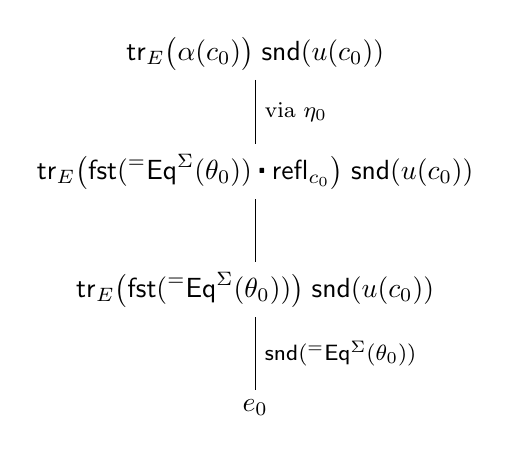
\begin{tikzpicture}
\node (N0) at (0,3) {$\trans_E\big(\alpha(c_0)\big) \; \snd(u(c_0))$};
\node (N1) at (0,1.5) {$\trans_E\big(\fst(\idtodpair(\theta_0)) \ct \refl_{c_0}\big) \; \snd(u(c_0))$};
\node (N2) at (0,0) {$\trans_E\big(\fst(\idtodpair(\theta_0))\big) \; \snd(u(c_0))$};
\node (N3) at (0,-1.5) {$e_0$};
\draw[-] (N0) -- node[right]{\footnotesize via $\eta_0$} (N1);
\draw[-] (N1) -- node[right]{\footnotesize} (N2);
\draw[-] (N2) -- node[right]{\footnotesize $\snd(\idtodpair(\theta_0))$} (N3);
\end{tikzpicture}
\end{center}
and $\phi_1$ is defined analogously.
\end{proof}

\begin{corollary}\label{lem:BoolMainInt}
In $\Hint$, the following conditions on an algebra $\X : \BoolAlg_{\UU_i}$ are equivalent:
\begin{enumerate}
\item $\X$ satisfies the induction principle on the universe $\UU_j$
\item $\X$ satisfies the recursion and recursion uniqueness principles on the universe $\UU_j$
\item $\X$ is homotopy-initial on the universe $\UU_j$  
\end{enumerate}
for $j \geq i$. In other words, we have \[ \HasBoolInd_{\UU_j}(\X)  \;\; \simeq \;\; \HasBoolRec_{\UU_j}(\X) \times \HasBoolRecUniq_{\UU_j}(\X) \;\; \simeq \;\; \IsBoolHInit_{\UU_j}(\X) \]
provided $j \geq i$. Furthermore, all 3 conditions are mere propositions.
\end{corollary}
\begin{proof}
Conditions (1) and (3) are mere propositions by Lem.~\ref{lem:IsContrIsProp} (for the latter), Lem.~\ref{lem:PropChar},~\ref{lem:BoolIndImpUniqInt} (for the former), and the fact that a family of mere propositions is itself a mere proposition.
\end{proof}

Furthermore, we have the following corollary which does \emph{not} have an analogue in the extensional case:
\begin{corollary}\label{BoolHInitIso}
In $\Hint$, any two algebras $\X,\Y : \BoolAlg_{\UU_i}$ which are homotopy-initial on $\UU_i$ are equal:
\[ \IsBoolHInit_{\UU_i}(\X) \to \IsBoolHInit_{\UU_i}(\Y) \to \X = \Y\] 
\end{corollary}
\begin{proof}
By Lem.~\ref{BoolAlgSpace} it suffices to construct an isomorphism between $\X$ and $\Y$. Since $\X$ and $\Y$ are both homotopy-initial on $\UU_i$, there exist homomorphisms $\mu : \BoolHom \; \X \; \Y$ and $\nu : \BoolHom \; \Y \; \X$. Again by homotopy-initiality, we have $\nu \comp \mu = \one_\X$ and $\mu \comp \nu = \one_\Y$, which gives us the desired isomorphism.
\end{proof}

We can thus characterize the type $\Bool$ using the universal property of homotopy-initiality as follows.
\begin{corollary}\label{lem:BoolInitInt}
In $\Hint$ extended with the type $\Bool$, the algebra $(\Bool,0,1) : \BoolAlg_{\UU_0}$ is homotopy-initial on any universe $\UU_j$.
\end{corollary}

\begin{corollary}\label{lem:BoolCharInt}
In $\Hint$ extended with an algebra $\X : \BoolAlg_{\UU_0}$ which is homotopy-initial on any universe $\UU_j$, the type $\Bool$ with propositional computation rules is definable. 
\end{corollary}
\begin{proof}
We have an algebra $\cdot \vdash \X : \BoolAlg_{\UU_0}$ such that for any $j$, there exists a term $\cdot \vdash h_j  : \IsBoolHInit_{\UU_j}(\X)$. Since the requirement $j \geq 0$ always holds, Cor.~\ref{lem:BoolMainInt} implies that for any $j$, we have a term $\cdot \vdash r_j : \HasBoolInd_{\UU_j}(\X)$. This implies that the type $\Bool$ with propositional computation rules is definable.
\end{proof}

Corollaries~\ref{lem:BoolCharInt} and \ref{lem:BoolInitInt} are the analogue in Homotopy Type Theory of the characterization of 
$\Bool$ as a strict coproduct $1+1$ in extensional type theory. It makes precise the rough idea that, 
in intensional type theory, $\Bool$ is a kind of homotopy coproduct or weak $\omega$-coproduct 
in the weak $\omega$-category $\mathcal{C}(\Hint)$ of types, terms, identity terms, higher identity terms, \ldots.  
It is worth emphasizing that homotopy-initiality is a purely type-theoretic notion; despite having an obvious semantic interpretation, it is formulated in terms of inhabitation of specific, definable types. Indeed, Corollary~\ref{lem:BoolMainInt} and its proof have been completely formalized in the Coq proof assistant~\cite{AwodeyS:indtht}.

%%%%%%%%%%%%%%%%%%%%%%%%%%%%%%%%%%%%%%%%%%%%%%%%%%%%%%%%%%%%%%%%%%%%%%%%%%%%%%%%%%%%%%%%%%%%%%%%%%%%%%%%%%
%%%%%%%%%%%%%%%%%%%%%%%%%%%%%%%%%%%%%%%%%%%%%%%%%%%%%%%%%%%%%%%%%%%%%%%%%%%%%%%%%%%%%%%%%%%%%%%%%%%%%%%%%% 

\subsection{W-types}\label{subsection:main}

\noindent Although it is more elaborate to state (and difficult to prove) owing to the presence of 
recursively generated data, our main result on  W-types is analogous to 
the foregoing example in the following respect: rather than being strict initial algebras, as in the 
extensional case, W-types with propositional computation rules are instead homotopy-initial algebras. This fact can again be stated 
entirely syntactically, as an equivalence between the definability of W-types with propositional computation rules (which we spell
out below) and the existence of a suitable family of homotopy-initial algebras.  Moreover, as in the simple case of the type $\Bool$ above, the proof is again entirely constructive.

The propositional computation rules for W-types are as follows:\smallskip
\begin{itemize}
\item Propositional $\W$-computation rule.\smallskip
\begin{mathpar}
\inferrule{A : \UU_i \\ x:A \vdash B(x) : \UU_i \\ a : A \\ t : B(a) \to \W \\ w : \W \vdash E(w) : \UU_j \\ x:A, p: B(x) \to \W, r : \prd{b:B(x)} E(p \;b) \vdash e(x,p,r) :E(\wsup(x,p))}
{\windcomp_{\UU_i}(A,x.B,w.E,x.p.r.e,a,t):\wind(\wsup(a,t)) = e(a,t,\lam{b:B(a)} \wind(t\;b))}
\end{mathpar}
\item Simple propositional $\W$-computation rule.\smallskip
\begin{mathpar}
\inferrule{A : \UU_i \\ x:A \vdash B(x) : \UU_i \\ a : A \\ t : B(a) \to \W \\ C : \UU_j \\ x:A, r : B(x) \to C \vdash c(x,r) : C}
{\wreccomp_{\UU_i}(A,x.B,C,x.r.c,a,t) : \wrec(\wsup(a,t)) = c(a,\lam{b:B(a)} \wrec(t \;b))}
\end{mathpar}
\end{itemize}\smallskip

\begin{remark}\label{thm:wtypesinvariance}
One interesting aspect of this group of rules is that, unlike the standard rules for $\W$-types, they are invariant under equivalence, and propositional equality in particular. 
If $A:\UU_i$ and $x:A \vdash B(x):\UU_i$ and we have a type $W : \UU_i$ such that $W \simeq \W^{\UU_i}_{x:A} B(x)$, then $W$ can be shown to satisfy the same rules as $\W^{\UU_i}_{x:A} B(x)$, in the sense that there are definable terms playing the role of the primitive constants that appear in the rules for $\W^{\UU_i}_{x:A} B(x)$.
\end{remark}

We again have uniqueness principles, in the propositional form:
\begin{itemize}
\item Propositional $\W$-uniqueness principle.\smallskip
\begin{mathpar}
\inferrule{A : \UU_i \\ x:A \vdash B(x) : \UU_i \\ m : \W \\ w:\W \vdash E(w) : \UU_j \\ x:A, p: B(x) \to \W, r : \prd{b:B(x)} E(p \;b) \vdash e(x,p,r) :E(\wsup(x,p)) \\ w:\W \vdash f(w) : E(w) \\ w:\W \vdash g(w) : E(w) \\ x:A, p: B(x) \to \W \vdash \gamma(x,p) : f(\wsup(x,p)) = e(x,p,\lam{b:B(x)} f(p \;b)) \\ x:A, p: B(x) \to \W \vdash \delta(x,p) : g(\wsup(x,p)) = e(x,p,\lam{b:B(x)} g(p \;b))}
{\winduniq_{\UU_i}(A,x.B,w.E,x.p.r.e,w.f,x.p.\gamma,w.g,x.p.\delta,m) : f(m) = g(m)}
\end{mathpar}
\item Simple propositional $\W$-uniqueness principle.\smallskip
\begin{mathpar}
\inferrule{A : \UU_i \\ x:A \vdash B(x) : \UU_i \\ m : \W \\ C : \UU_j \\ x:A, r : B(x) \to C \vdash c(x,r) : C \\ w:\W\vdash f(w) : C \\ x:A, p: B(x) \to \W \vdash \gamma(x,p) : f(\wsup(x,p)) = c(x,\lam{b:B(x)} f(p \;b)) \\ w:\W\vdash g(x) : C \\ x:A, p: B(x) \to \W \vdash \delta(x,p) : g(\wsup(x,p)) = c(x,\lam{b:B(x)} g(p \;b))}
{\wrecuniq_{\UU_i}(A,x.B,C,x.r.c,w.f,x.p.\gamma,w.g,x.p.\delta,m) : f(m) = g(m)}
\end{mathpar}
\end{itemize} \smallskip
The witness terms will be shortened to $\winduniq(m), \wrecuniq(m)$ where appropriate. In showing the above laws, we proceed analogously to the extensional case: we use the induction principle with the type family $x \mapsto f(w) =_{E(w)} g(w)$. For this we need to show that for any $x,p$ we have $f(\wsup(x,p)) = g(\wsup(x,p))$ under the induction hypothesis $h : \prd{b:B(x)} f(p\;b) = g(p\;b)$. We can construct this path explicitly as 
\[ \gamma(x,p) \ct \app_{e(x,p,-)}(\funext(h))\ct \delta(x,p)^{-1} \]
The simple uniqueness rule again follows from the dependent one. Invoking the corresponding (propositional) computation rule, we  get the following coherence principles for W-types:
\begin{itemize}
\item Propositional $\W$-coherence principle.\smallskip
\begin{mathpar}
\inferrule{A : \UU_i \\ x:A \vdash B(x) : \UU_i \\ a : A \\ t : B(a) \to \W \\ w:\W \vdash E(w) : \UU_j \\ x:A, p: B(x) \to \W, r : \prd{b:B(x)} E(p \;b) \vdash e(x,p,r) :E(\wsup(x,p)) \\ w:\W \vdash f(w) : E(w) \\ w:\W \vdash g(w) : E(w) \\ x:A, p: B(x) \to \W \vdash \gamma(x,p) : f(\wsup(x,p)) = e(x,p,\lam{b:B(x)} f(p \;b)) \\ x:A, p: B(x) \to \W \vdash \delta(x,p) : g(\wsup(x,p)) = e(x,p,\lam{b:B(x)} g(p \;b))}
{\windcoh_{\UU_i}(A,x.B,w.E,x.p.r.e,w.f,x.p.\gamma,w.g,x.p.\delta,a,t) : \\ \winduniq(\wsup(a,t)) = \gamma(a,t) \ct \app_{e(a,t,-)}(\funext(\lam{b:B(a)}\winduniq(t\;b)))\ct \delta(a,t)^{-1}}
\end{mathpar}
\item Simple propositional $\W$-coherence principle.\smallskip
\begin{mathpar}
\inferrule{A : \UU_i \\ x:A \vdash B(x) : \UU_i \\ a : A \\ t : B(a) \to \W \\ C : \UU_j \\ x:A, r : B(x) \to C \vdash c(x,r) : C \\ w:\W\vdash f(w) : C \\ x:A, p: B(x) \to \W \vdash \gamma(x,p) : f(\wsup(x,p)) = c(x,\lam{b:B(x)} f(p \;b)) \\ w:\W\vdash g(x) : C \\ x:A, p: B(x) \to \W \vdash \delta(x,p) : g(\wsup(x,p)) = c(x,\lam{b:B(x)} g(p \;b))}
{\wreccoh_{\UU_i}(A,x.B,C,x.r.c,w.f,x.p.\gamma,w.g,x.p.\delta,a,t) : \\ \wrecuniq(\wsup(a,t)) = \gamma(a,t) \ct \app_{c(a,-)}(\funext(\lam{b:B(a)}\wrecuniq(t\;b)))\ct \delta(a,t)^{-1}}
\end{mathpar}
\end{itemize} \smallskip
This motivates the following definitions:

\begin{definition}\label{def:WCell}
For $A:\UU_i$, $B : A \to \UU_i$, $\X : \WAlg_{\UU_j}(A,B)$, $\Y : \WAlg_{\UU_k}(A,B)$ and homomorphisms $\mu, \nu : \WHom \; \X \; \Y$, define the type of \emph{2-cells} between $\mu$ and $\nu$ by
\begin{align*} & \WCell \; (C,c) \; (D,d) \; (f,\gamma) \; (g,\delta) \defeq \\ & \;\;\; \;\;\;\WFibHom \; (C,c) \; \Big(f \sim g; x,p,r \mapsto \gamma(x,p) \ct \app_{d(x)}(\funext(r)) \ct \delta(x,p)^{-1}\Big)
\end{align*}
\end{definition}

\begin{definition}\label{def:WFibCell}
For $A:\UU_i$, $B : A \to \UU_i$, $\X : \WAlg_{\UU_j}(A,B)$, $\Y : \WFibAlg_{\UU_k}(A,B) \; \X$ and fibered homomorphisms $\mu, \nu : \WFibHom \; \X \; \Y$, define the type of \emph{fibered 2-cells} between $\mu$ and $\nu$ by
\begin{align*} & \WFibCell \; (C,c) \; (E, e) \; (f,\gamma) \; (g,\delta) \defeq \\ & \;\;\; \;\;\;\WFibHom \; (C,c) \; \Big(f \sim g; x,p,r \mapsto \gamma(x,p) \ct \app_{e(x,p)}(\funext(r)) \ct \delta(x,p)^{-1}\Big)
\end{align*}
\end{definition}
For brevity, we will often leave out the first two arguments. As expected, we have:
\begin{definition}\label{def:WHInit}
Given $A:\UU_i$, $B : A \to \UU_i$, an algebra $\X : \WAlg_{\UU_j}(A,B)$ is called \emph{homotopy-initial} on a universe $\UU_k$ if for any algebra $\Y : \WAlg_{\UU_k}(A,B)$, the type of $\W$-homomorphisms between $\X$ and $\Y$ is contractible:
\[ \IsWHInit_{\UU_k}(\X) \defeq \prd{(\Y:\WAlg_{\UU_k}(A,B))} \iscontr(\WHom \; \X \; \Y) \]  
\end{definition}

\begin{definition}
For $A:\UU_i$, $B : A \to \UU_i$, $\X : \WAlg_{\UU_j}(A,B)$ there is a designated \emph{identity} homomorphism from $\X$ to itself, defined by
\[ \WIdHom \; (C,c) \defeq (\idfun{C}; a,t \mapsto \refl_{c(a,t)}) \]
\end{definition}
As before, we denote this homomorphism by $\one_\X$.

\begin{definition}
For $A:\UU_i$, $B : A \to \UU_i$, $\X : \WAlg_{\UU_j}(A,B)$, $\Y : \WAlg_{\UU_k}(A,B)$, $\Z : \WAlg_{\UU_l}(A,B)$ and homomorphisms $\mu : \WHom \; \X \; \Y$, $\nu : \WHom \; \Y \; \Z$, the \emph{composition} of $\mu$ and $\nu$ is a homomorphism from $\X$ to $\Z$ defined by
\begin{align*} & \WCompHom \; (C,c) \; (D,d) \; (E,e) \; (f,\gamma) \; (g,\delta) \defeq  \Big(g \comp f; a,t \mapsto \app_g(\gamma(a,t)) \ct \delta(a, f \comp t) \Big)
\end{align*}
\end{definition}
As before, we often leave out the first three arguments and denote the composition by $\nu \comp \mu$.

\begin{definition}
For $A:\UU_i$, $B : A \to \UU_i$, $\X : \WAlg_{\UU_j}(A,B)$, $\Y : \WAlg_{\UU_k}(A,B)$ we define the type of \emph{isomorphisms} between $\X$ and $\Y$ as
\[\WAlgIso \; \X \; \Y \defeq \sm{(\rho : \WHom \; \X \; \Y)} \Big(\sm{(\mu : \WHom \; \Y \; \X)} \mu \comp \rho = \one_\X \Big) \times \Big(\sm{(\nu : \WHom \; \Y \; \X)} \rho \comp \nu = \one_\Y \Big) \] 
\end{definition}

\begin{lemma}\label{WFibHomSpace}
For $A:\UU_i$, $B : A \to \UU_i$, $\X : \WAlg_{\UU_j}(A,B)$, $\Y : \WFibAlg_{\UU_k}(A,B) \; \X$ and $\mu,\nu : \WFibHom \; \X \; \Y$, the path space $\mu = \nu$ is equivalent to the space of fibered 2-cells between $\mu$ and $\nu$:
\[ \mu = \nu \;\; \simeq \;\; \WFibCell \; \mu \; \nu \] 
\end{lemma}
\begin{proof}
Let algebras $(C,c) : \WAlg_{\UU_j}(A,B)$, $(E,e) : \WFibAlg_{\UU_k}(A,B) \; (C,c)$ and homomorphisms $(f,\gamma), (g,\delta) : \WFibHom \; (C,c) \; (E,e)$ be given. We have
\begin{alignat*}{4}
& (f,\gamma) = (g,\delta) & \simeq \\
& \sm{\alpha : f = g} \Big(\delta = \trans_{\big(h \mapsto \prd{a}\prd{t} h(c(a,t)) = e(a,t,\lam{b} h(t\;b))\big)}(\alpha) \; \gamma\Big) & \simeq \\
& \sm{\alpha : f = g} \Big(\delta = \lam{a} \lam{t} \happly(\alpha,c(a,t))^{-1} \ct \gamma(a,t) \ct \app_{e(a,t)}(\funext (\lam{b}\happly(\alpha,t \; b))) \Big) & \;\;\; \simeq \\
& \sm{\alpha : f \sim g} \Big(\delta = \lam{a} \lam{t} \; \alpha(c(a,t))^{-1} \ct \gamma(a,t) \ct \app_{e(a,t)}(\funext (\lam{b}\; \alpha(t \; b))) \Big) & \simeq \\
& \sm{\alpha : f \sim g} \prd{a}\prd{t}\Big(\delta(a,t) = \alpha(c(a,t))^{-1} \ct \gamma(a,t) \ct \app_{e(a,t)}(\funext (\lam{b}\; \alpha(t \; b))) \Big) & \simeq \\ 
& \sm{\alpha : f \sim g} \prd{a}\prd{t}\Big(\alpha(c(a,t)) = \gamma(a,t) \ct \app_{e(a,t)}(\funext (\lam{b}\; \alpha(t \; b))) \ct \delta(a,t)^{-1} \Big) & \equiv \\ 
& \WFibCell \; (f,\gamma) \; (g,\delta)
\end{alignat*}
\end{proof}

\begin{corollary}\label{WHomSpace}
For $A:\UU_i$, $B : A \to \UU_i$, $\X : \WAlg_{\UU_j}(A,B)$, $\Y : \WAlg_{\UU_k}(A,B)$ and $\mu,\nu : \WHom \; \X \; \Y$, the path space $\mu = \nu$ is equivalent to the space of 2-cells between $\mu$ and $\nu$:
\[ \mu = \nu \;\; \simeq \;\; \WCell \; \mu \; \nu \] 
\end{corollary}

\begin{lemma}\label{WAlgSpace}
Given $A:\UU_i$, $B : A \to \UU_i$ and $\X,\Y : \WAlg_{\UU_j}(A,B)$, the path space $\X = \Y$ is equivalent to the space of isomorphisms between $\X$ and $\Y$:
\[ \X = \Y \;\; \simeq \;\; \WAlgIso \; \X \; \Y \] 
\end{lemma}
\begin{proof}
Let algebras $(C,c), (D,d) : \WAlg_{\UU_j}(A,B)$ be given. We have
\begin{alignat*}{4}
& \WAlgIso \; (C,c) \; (D,d) & \equiv \\
& \sm{\rho : \big(\sm{f:C\to D} \prd{a}\prd{t} f(c(a,t)) = d(a,f \comp t) \big)} \Big(\sm{\mu : \big(\sm{g:D\to C} \prd{a}\prd{s} g(d(a,s)) = c(a,g \comp s)\big)} \mu \comp \rho = \one_{(C,c)} \Big)\; \times & \\
& \;\;\;\;\;\;\;\;\;\;\;\;\;\;\;\;\;\;\;\;\;\;\;\;\;\;\;\;\;\;\;\;\;\;\;\;\;\;\;\;\;\;\;\;\;\;\;\;\;\;\Big(\sm{\nu : \big(\sm{h:D\to C} \prd{a}\prd{s} h(d(a,s))=c(a,h\comp s)\big)} \rho \comp \nu = \one_{(D,d)}\Big) & \;\;\;\;\;\;\; \simeq \\
& \sm{f : C\to D} \sm{\epsilon : (\prd{a}\prd{t} f(c(a,t)) = d(a,f \comp t))} \Big(\sm{g:D\to C} \sm{\gamma : (\prd{a}\prd{s} g(d(a,s)) = c(a,g \comp s))} P_{f,\epsilon,g,\gamma}\Big) \; \times & \\
& \;\;\;\;\;\;\;\;\;\;\;\;\;\;\;\;\;\;\;\;\;\;\;\;\;\;\;\;\;\;\;\;\;\;\;\;\;\;\;\;\;\;\;\;\;\;\;\;\;\; \Big(\sm{h:D\to C} \sm{\delta : (\prd{a}\prd{s} h(d(a,s))=c(a,h\comp s))} Q_{f,\epsilon,h,\delta} \Big) &
\end{alignat*}
where
\begin{align*}
& P_{f,\epsilon,g,\gamma} \defeq \Big(g \comp f; a,t \mapsto \app_g(\epsilon(a,t)) \ct \gamma(a, f \comp t)\Big) = \Big(\idfun{C}; a,t \mapsto \refl_{c(a,t)}\Big) \\
& Q_{f,\epsilon,h,\delta} \defeq \Big(f \comp h; a,s \mapsto \app_f(\delta(a,s)) \ct \epsilon(a, h \comp t)\Big) = \Big(\idfun{D}; a,s \mapsto \refl_{d(a,s)}\Big)
\end{align*}
Now we have
\begin{alignat*}{4}
& P_{f,\epsilon,g,\gamma} & \equiv \\
& \Big(g \comp f; a,t \mapsto \app_g(\epsilon(a,t)) \ct \gamma(a, f \comp t)\Big) = \Big(\idfun{C}; a,t \mapsto \refl_{c(a,t)}\Big) & \simeq \\
& \sm{\alpha : g \comp f = \idfun{C}} \Big(\lam{a}\lam{t} \app_g(\epsilon(a,t)) \ct \gamma(a, f \comp t)\Big) = \trans^{-1}_{\big(i \mapsto \prd{a}\prd{t} i(c(a,t)) = c(a,i \comp t)\big)}(\alpha) \; \Big(\lam{a}\lam{t} \refl_{c(a,t)}\Big) & \;\;\; \simeq \\
& \sm{\alpha : g \comp f = \idfun{C}} \Big(\lam{a}\lam{t} \app_g(\epsilon(a,t)) \ct \gamma(a, f \comp t)\Big) = \lam{a}\lam{t} & \\ & \;\;\;\;\;\;\; \happly(\alpha, c(a,t)) \ct \refl_{c(a,t)} \ct \Big(\app_{c(a)}(\funext(\lam{b} \happly(\alpha, t\;b)))\Big)^{-1} & \;\;\; \simeq \\
& \sm{\alpha : g \comp f = \idfun{C}} \prd{a}\prd{t} \Big(\app_g(\epsilon(a,t)) \ct \gamma(a, f \comp t)\Big) = & \\
& \;\;\;\;\;\;\; \happly(\alpha, c(a,t)) \ct \refl_{c(a,t)} \ct \Big(\app_{c(a)}(\funext(\lam{b} \happly(\alpha, t\;b)))\Big)^{-1} & \;\;\; \simeq \\
& \sm{\alpha : g \comp f \sim \idfun{C}} \prd{a}\prd{t} \Big(\app_g(\epsilon(a,t)) \ct \gamma(a, f \comp t)\Big) = & \\
& \;\;\;\;\;\;\; \alpha(c(a,t)) \ct \refl_{c(a,t)} \ct \Big(\app_{c(a)}(\funext(\lam{b} \; \alpha(t\;b)))\Big)^{-1} & \;\;\; \simeq \\
& \sm{\alpha : g \comp f \sim \idfun{C}} \prd{a}\prd{t} \Big(\alpha(c(a,t)) = \app_g(\epsilon(a,t)) \ct \gamma(a, f \comp t) \ct \app_{c(a)}(\funext(\lam{b} \; \alpha(t\;b)))\Big) &
\end{alignat*}
and analogously
\begin{alignat*}{4}
Q_{f,\epsilon,h,\delta} \simeq \sm{\beta : f \comp h \sim \idfun{D}} \prd{a}\prd{s} \Big(\beta(d(a,s)) = \app_f(\delta(a,s)) \ct \epsilon(a, h \comp s) \ct \app_{d(a)}(\funext(\lam{b} \; \beta(s\;b)))\Big) &
\end{alignat*}
Thus we can express $\WAlgIso \; (C,c) \; (D,d)$ equivalently as the type
\begin{alignat*}{4}
& \sm{f : C\to D} \sm{\epsilon : (\prd{a}\prd{t} f(c(a,t)) = d(a,f \comp t))} \sm{g:D\to C} \sm{\alpha : g \comp f \sim \idfun{C}} \sm{h:D \to C} \sm{\beta : f \comp h \sim \idfun{D}} R_{f,\epsilon,g,\alpha} \times S_{f,\epsilon,h,\beta}
\end{alignat*}
where
\begin{alignat*}{4}
& R_{f,\epsilon,g,\alpha} \defeq \sm{\gamma : (\prd{a}\prd{s} g(d(a,s)) = c(a,g \comp s))} \prd{a}\prd{t} \\ & \;\;\;\;\;\;\;\;\;\;\;\; \alpha(c(a,t)) = \app_g(\epsilon(a,t)) \ct \gamma(a, f \comp t) \ct \app_{c(a)}(\funext(\lam{b} \; \alpha(t\;b))) \\
& S_{f,\epsilon,h,\beta} \defeq \sm{\delta : (\prd{a}\prd{s} h(d(a,s)) = c(a,h \comp s))} \prd{a}\prd{s} \\ & \;\;\;\;\;\;\;\;\;\;\;\; \beta(d(a,s)) = \app_f(\delta(a,s)) \ct \epsilon(a, h \comp s) \ct \app_{d(a)}(\funext(\lam{b} \; \beta(s\;b)))
\end{alignat*}
Now we have
\begin{alignat*}{4}
& S_{f,\epsilon,h,\beta} & \equiv \\
& \sm{\delta : (\prd{a}\prd{s} h(d(a,s)) = c(a,h \comp s))} \prd{a}\prd{s} & \\
& \;\;\;\;\;\;\;\;\;\; \beta(d(a,s)) = \app_f(\delta(a,s)) \ct \epsilon(a, h \comp s) \ct \app_{d(a)}(\funext(\lam{b} \; \beta(s\;b))) & \;\;\; \simeq \\
& \prd{a}\prd{s}\sm{\delta : h(d(a,s)) = c(a,h \comp s)}  & \\
& \;\;\;\;\;\;\;\;\;\; \beta(d(a,s)) = \app_f(\delta) \ct \epsilon(a, h \comp s) \ct \app_{d(a)}(\funext(\lam{b} \; \beta(s\;b))) & \;\;\; \simeq \\
& \prd{a}\prd{s}\sm{\delta : h(d(a,s)) = c(a,h \comp s)}  & \\
& \;\;\;\;\;\;\;\;\;\; \app_f(\delta) = \beta(d(a,s)) \ct \Big(\app_{d(a)}(\funext(\lam{b} \; \beta(s\;b)))\Big)^{-1} \ct \epsilon(a, h \comp s)^{-1} & \;\;\; \simeq \\
& \prd{a}\prd{s}\one & \;\;\; \simeq \\
& \one
\end{alignat*}
by Lem.~\ref{lem_singl_equiv_contr},~\ref{lem_ap_equiv}, and the fact that $g,\alpha,h,\beta$ make $f$ into an equivalence. This last fact also implies that the mapping $t \mapsto f \comp t$ is an equivalence between $B(a) \to C$ and $B(a) \to D$ by Lem.~\ref{lem_equiv_comp}\ednote{Which says that if $f:B \to C$ is an equivalence, then so is the mapping $h \mapsto f \comp h$ between $A \to B$ and $A \to C$}. Thus the mapping $\gamma \mapsto \lam{a}\lam{t} \gamma(a,f \comp t)$ is an equivalence between the types $\prd{a:A}\prd{s:B(a)\to D} g(d(a,s)) = c(a,g \comp s)$ and $\prd{a:A}\prd{t:B(a)\to C} g(d(a,f \comp t)) = c(a,g \comp f \comp t)$. Thus:
\begin{alignat*}{4}
& R_{f,\epsilon,g,\alpha} & \equiv \\
& \sm{\gamma : \big(\prd{a}\prd{s} g(d(a,s)) = c(a,g \comp s)\big)} \prd{a}\prd{t} & \\ 
& \;\;\;\;\;\;\;\;\;\; \alpha(c(a,t)) = \app_g(\epsilon(a,t)) \ct \gamma(a, f \comp t) \ct \app_{c(a)}(\funext(\lam{b} \; \alpha(t\;b))) & \;\;\; \simeq \\
& \sm{\gamma : \big(\prd{a}\prd{t} g(d(a,f \comp t)) = c(a,g \comp f \comp t)\big)} \prd{a}\prd{t} & \\ 
& \;\;\;\;\;\;\;\;\;\; \alpha(c(a,t)) = \app_g(\epsilon(a,t)) \ct \gamma(a,t) \ct \app_{c(a)}(\funext(\lam{b} \; \alpha(t\;b))) & \;\;\; \simeq \\
& \prd{a}\prd{t} \sm{\gamma : g(d(a,f \comp t)) = c(a,g \comp f \comp t)} & \\ 
& \;\;\;\;\;\;\;\;\;\; \alpha(c(a,t)) = \app_g(\epsilon(a,t)) \ct \gamma \ct \app_{c(a)}(\funext(\lam{b} \; \alpha(t\;b))) & \;\;\; \simeq \\
& \prd{a}\prd{t} \sm{\gamma : g(d(a,f \comp t)) = c(a,g \comp f \comp t)} & \\ 
& \;\;\;\;\;\;\;\;\;\; \gamma = \Big(\app_g(\epsilon(a,t))\Big)^{-1} \ct \alpha(c(a,t)) \ct \Big(\app_{c(a)}(\funext(\lam{b} \; \alpha(t\;b)))\Big)^{-1} & \;\;\; \simeq \\
& \prd{a}\prd{t}\one & \;\;\; \simeq \\
& \one
\end{alignat*}
by Lem.~\ref{lem_singl_contr}. Thus, we have
\begin{alignat*}{4}
& \WAlgIso \; (C,c) \; (D,d) & \simeq \\
& \sm{f : C\to D} \sm{g:D\to C} \sm{\alpha : g \comp f \sim \idfun{C}} \sm{h:D \to C} \sm{\beta : f \comp h \sim \idfun{D}} \prd{a}\prd{t} f(c(a,t)) = d(a,f \comp t) & \;\;\; \simeq \\
& \sm{f : C\to D} \isequiv(f) \times \prd{a}\prd{t} f(c(a,t)) = d(a,f \comp t) & \;\;\; \simeq \\
& \sm{p : C \simeq D} \prd{a}\prd{t} \big(\fst(p) \; c(a,t)\big) = d(a, \fst(p) \comp t) & \;\;\; \simeq \\
& \sm{p : C = D} \prd{a}\prd{t} \Big(\fst(\idtoeq(p)) \; c(a,t)\Big) = d\Big(a, \fst(\idtoeq(p)) \comp t\Big) & \;\;\; \equiv \\
& \sm{p : C = D} \prd{a} \prd{t} \Big(\trans_{X \mapsto X}(p) \; c(a,t) = d\Big(a,\fst(\idtoeq(p)) \comp t\Big)\Big) & \simeq \\
& \sm{p : C = D} \prd{a} \prd{t} \Big(c(a,t) = \trans^{-1}_{X \mapsto X}(p) \; d\Big(a,\fst(\idtoeq(p)) \comp t\Big)\Big) & \simeq \\
& \sm{p : C = D} \Big(c = \lam{a}\lam{t}\trans^{-1}_{X \mapsto X}(p) \; d\Big(a,\fst(\idtoeq(p)) \comp t\Big)\Big) & \simeq \\ 
& \sm{p : C = D} \Big(c = \trans^{-1}_{\big(X \mapsto \prd{a:A} (B(a) \to X) \to X\big)}(p) \; d\Big) & \simeq \\ 
& (C,c) = (D,d)
\end{alignat*}
\end{proof}

As desired, the analogues of the lemmas from section \ref{subsection:wtypes} still hold in the setting of homotopy type theory:

\begin{lemma}\label{lem:WIndImpUniqInt}
In $\Hint$, for $A:\UU_i$, $B : A \to \UU_i$, if an algebra $\X : \WAlg_{\UU_j}(A,B)$ satisfies the induction principle on the universe $\UU_k$, it also satisfies the induction uniqueness principle on $\UU_k$. In other words, we have
\[ \HasWInd_{\UU_k}(\X) \;\; \rightarrow \;\; \HasWIndUniq_{\UU_k}(\X) \]
\end{lemma}
\begin{proof}
Let an algebra $(C,c) : \WAlg_{\UU_j}(A,B)$ be given. To prove the induction uniqueness principle, take any algebra $(E,e) : \WFibAlg_{\UU_k}(A,B) \; (C,c)$ and homomorphisms $(f,\gamma), (g,\delta) : \WFibHom \; (C,c) \; (E,e)$. By Lem.~\ref{WFibHomSpace}, to show $(f,\gamma) = (g,\delta)$ it suffices to exhibit a fibered 2-cell between $(f,\gamma)$ and $(g,\delta)$. For this we use the induction principle with the fibered algebra $\Big(f \sim g; x,p,r \mapsto \gamma(x,p) \ct \app_{e(x,p)}(\funext(r)) \ct \delta(x,p)^{-1}\Big)$ and we are done.
\end{proof}

%\begin{lemma}\label{lem:WRecUniqEqInitInt}
%In $\Hint$, for $A:\UU_i$, $B : A \to \UU_i$ the following conditions on an algebra $\X : \WAlg_{\UU_j}(A,B)$ are equivalent:
%\begin{enumerate}
%\item $\X$ satisfies the recursion and recursion uniqueness principles on the universe $\UU_k$
%\item $\X$ is homotopy-initial on the universe $\UU_k$
%\end{enumerate}
%In other words, we have
%\[ \HasWRec_{\UU_k}(\X) \times \HasWRecUniq_{\UU_k}(\X) \;\; \simeq \;\; \IsWHInit_{\UU_k}(\X) \]
%\end{lemma}
%\begin{proof}
%By Lem.~\ref{lem:ContrChar}.
%\end{proof}

\begin{corollary}\label{lem:WIndImpHInitInt}
In $\Hint$, for $A:\UU_i$, $B : A \to \UU_i$, if an algebra $\X : \WAlg_{\UU_j}(A,B)$ satisfies the induction principle on the universe $\UU_k$, it is homotopy-initial on $\UU_k$. In other words, we have
\[ \HasWInd_{\UU_k}(\X) \;\; \rightarrow \;\; \IsWHInit_{\UU_k}(\X) \]
\end{corollary}

\begin{lemma}\label{lem:WRecUniqImpIndInt}
In $\Hint$, for $A:\UU_i$, $B : A \to \UU_i$, if an algebra $\X : \WAlg_{\UU_j}(A,B)$ satisfies the recursion and recursion uniqueness principles on the universe $\UU_k$ and $k \geq j$, then it satisfies the induction principle on $\UU_k$. In other words, we have
\[ \HasWRec_{\UU_k}(\X) \times \HasWRecUniq_{\UU_k}(\X) \;\; \rightarrow \; \; \HasWInd_{\UU_k}(\X) \]
provided $k \geq j$.
\end{lemma}
\begin{proof}
Let algebras $(C,c) : \WAlg_{\UU_j}(A,B)$ and $(E,e) : \WFibAlg_{\UU_k} \; (C,c)$ be given. We use the recursion principle with the algebra $(\sm{x:C} E(x); a,s \mapsto d(a,s))$ where
\[ d(a,s) \defeq \Big(c\big(a,\lam{b:B(a)} \fst(s\;b)\big), e\big(a, \lam{b:B(a)} \fst(s\;b), \lam{b:B(a)} \snd(s\;b)\big) \Big) \]
We note that the carrier type belongs to $\UU_k$ as $j \leq k$. This gives us a homomorphism $(u,\theta)$, where $u : C \to \sm{x:C} E(x)$ and $\theta : \prd{a:A}\prd{t:B(a)\to C} u(c(a,t)) = d(a,\lam{b:B(a)}u(t\;b))$. We can now form two homomorphisms 
\[\Big(\fst \comp u; a,t \mapsto \fst(\idtodpair(\theta(a,t)))\Big), \Big(\idfun{C}; a,t \mapsto \refl_{c(a,t)}\Big) : \WHom \; (C,c) \; (C,c)\]
The recursion uniqueness principle tells us that these homomorphisms are equal. By Cor.~\ref{WHomSpace} this means there exists a 2-cell $(\alpha,\eta)$ between them, i.e., we have 
\begin{align*}
& \alpha : \fst \comp u \sim \idfun{C} \\
& \eta : \prd{a:A}\prd{t:B(a)\to C} \Big(\alpha(c(a,t)) = \fst(\idtodpair(\theta(a,t))) \ct \app_{c(a)}\big(\funext(\lam{b:B(a)} \alpha(t\;b))\big) \ct \refl_{c(a,t)}\Big)
\end{align*}
Now it is easy to see that for any $a : A$, path $p : t_1 =_{B(a) \to C} t_2$, and $s : \prd{b:B(a)} E(t_1 \; b)$, we have a higher path
\[ \epsilon(a,p,s) : \trans_E\big(\app_{c(a)}(p)\big) \; e(a,t_1,s) = e\Big(a,t_2,\big(\lam{b:B(a)} \trans_E(\happly(p,b)) \; (s \; b)\big)\Big) \] 
To show this, we simply use path induction on $p$.

We can thus define the desired fibered homomorphism as \[\Big(x \mapsto \trans_E(\alpha(x)) \; \snd(u(x)); a,t \mapsto \phi(a,t) \Big) : \WFibHom \; (C,c) \; (E,e)\]
where $\phi(a,t)$ is the path
\begin{center}
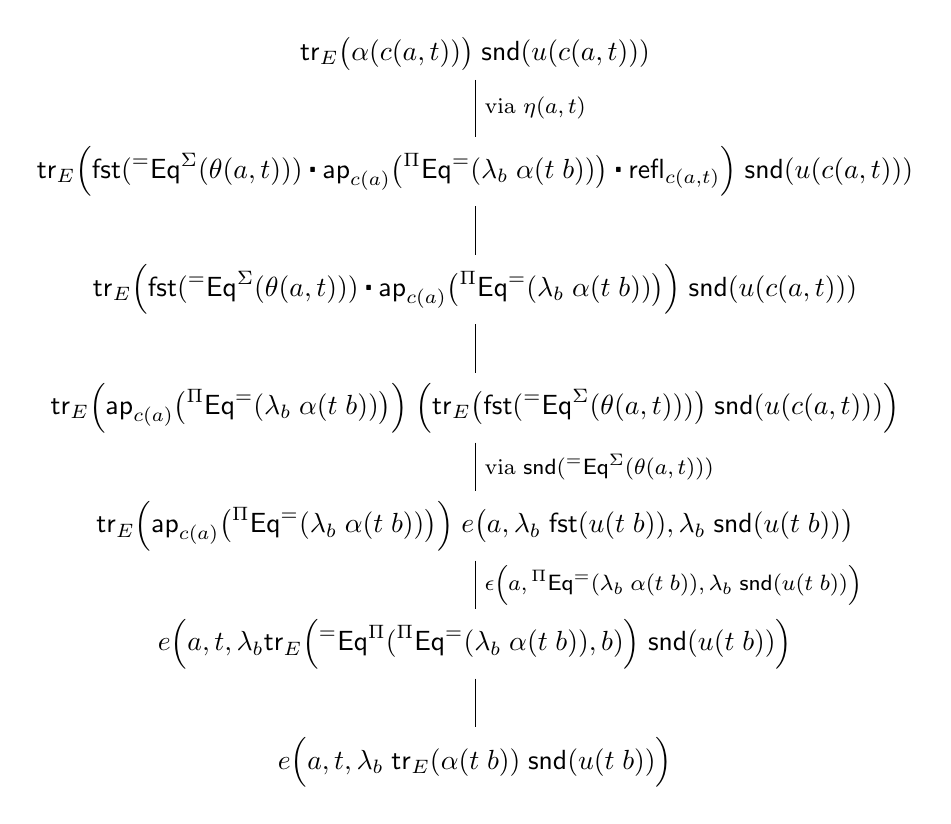
\begin{tikzpicture}
\node (N0) at (0,12) {$\trans_E\big(\alpha(c(a,t))\big) \; \snd(u(c(a,t)))$};
\node (N1) at (0,10.5) {$\trans_E\Big(\fst(\idtodpair(\theta(a,t))) \ct \app_{c(a)}\big(\funext(\lam{b}\; \alpha(t\;b))\big) \ct \refl_{c(a,t)}\Big) \; \snd(u(c(a,t)))$};
\node (N2) at (0,9) {$\trans_E\Big(\fst(\idtodpair(\theta(a,t))) \ct \app_{c(a)}\big(\funext(\lam{b} \;\alpha(t\;b))\big)\Big) \; \snd(u(c(a,t)))$};
\node (N3) at (0,7.5) {$\trans_E\Big(\app_{c(a)}\big(\funext(\lam{b} \; \alpha(t\;b))\big)\Big) \; \Big(\trans_E\big(\fst(\idtodpair(\theta(a,t)))\big) \; \snd(u(c(a,t)))\Big)$};
\node (N4) at (0,6) {$\trans_E\Big(\app_{c(a)}\big(\funext(\lam{b}\; \alpha(t\;b))\big)\Big) \; e\big(a, \lam{b} \;\fst(u(t\;b)), \lam{b}\; \snd(u(t\;b))\big) $};
\node (N5) at (0,4.5) {$e\Big(a,t,\lam{b} \trans_E\Big(\happly(\funext(\lam{b}\; \alpha(t\;b)),b)\Big) \; \snd(u(t\;b))\Big)$};
\node (N6) at (0,3) {$e\Big(a,t,\lam{b} \; \trans_E(\alpha(t\;b)) \; \snd(u(t\;b))\Big)$};

\draw[-] (N0) -- node[right]{\footnotesize via $\eta(a,t)$} (N1);
\draw[-] (N1) -- node[right]{\footnotesize} (N2);
\draw[-] (N2) -- node[right]{\footnotesize} (N3);
\draw[-] (N3) -- node[right]{\footnotesize via $\snd(\idtodpair(\theta(a,t)))$} (N4);
\draw[-] (N4) -- node[right]{\footnotesize $\epsilon\Big(a,\funext(\lam{b} \; \alpha(t\;b)), \lam{b} \; \snd(u(t\;b))\Big)$} (N5);
\draw[-] (N5) -- node[right]{\footnotesize} (N6);
\end{tikzpicture}
\end{center}
\end{proof}

\begin{corollary}\label{lem:WMainInt}
In $\Hint$, for $A:\UU_i$, $B : A \to \UU_i$, the following conditions on an algebra $\X : \WAlg_{\UU_j}(A,B)$ are equivalent:
\begin{enumerate}
\item $\X$ satisfies the induction principle on the universe $\UU_k$
\item $\X$ satisfies the recursion and recursion uniqueness principles on the universe $\UU_k$
\item $\X$ is homotopy-initial on the universe $\UU_k$  
\end{enumerate}
for $k \geq j$. In other words, we have \[ \HasWInd_{\UU_k}(\X)  \;\; \simeq \;\; \HasWRec_{\UU_k}(\X) \times \HasWRecUniq_{\UU_k}(\X) \;\; \simeq \;\; \IsWHInit_{\UU_k}(\X) \]
provided $j \geq i$. Furthermore, all 3 conditions are mere propositions.
\end{corollary}
\begin{proof}
Conditions (1) and (3) are mere propositions by Lem.~\ref{lem:IsContrIsProp} (for the latter), Lem.~\ref{lem:PropChar},~\ref{lem:WIndImpUniqInt} (for the former), and the fact that a family of mere propositions is itself a mere proposition.
\end{proof}

As in the case of the type $\Bool$, we have the following corollary:
\begin{corollary}\label{WHInitIso}
In $\Hint$, for $A:\UU_i$, $B : A \to \UU_i$, two algebras $\X,\Y : \WAlg_{\UU_j}(A,B)$ which are homotopy-initial on $\UU_j$ are equal:
\[ \IsWHInit_{\UU_j}(\X) \to \IsWHInit_{\UU_j}(\Y) \to \X = \Y\] 
\end{corollary}
\begin{proof}
By Lem.~\ref{WAlgSpace} it suffices to construct an isomorphism between $\X$ and $\Y$. Since $\X$ and $\Y$ are both homotopy-initial on $\UU_j$, there exist homomorphisms $\mu : \WHom \; \X \; \Y$ and $\nu : \WHom \; \Y \; \X$. Again by homotopy-initiality, we have $\nu \comp \mu = \one_\X$ and $\mu \comp \nu = \one_\Y$, which gives us the desired isomorphism.
\end{proof}

We can thus characterize $\W$-types using the universal property of initiality as follows.
\begin{corollary}\label{lem:WInitInt}
In $\Hint$ with $\W$-types, for any $A:\UU_i$, $B : A \to \UU_i$, the algebra \[\Big(\W^{\UU_i}_{x:A}B(x),\lam{a}\lam{t} \wsup_{\UU_i}^{A,x.B(x)}(a,t) \Big) : \WAlg_{\UU_i}(A,B)\] is homotopy-initial on any universe $\UU_j$.
\end{corollary}

\begin{corollary}\label{lem:WCharInt}
In $\Hint$ extended with an algebra $\X_{\UU_i}(A,B) : \WAlg_{\UU_i}(A,B)$ for any $\UU_i$, $A : \UU_i$, $B : A \to \UU_i$, which is homotopy-initial on any universe $\UU_j$, Martin-L{\"o}f's $\W$-types are definable.
\end{corollary}
\begin{proof}
For any $i$, the algebra $A:\UU_i,B:A\to \UU_i \vdash \X_{\UU_i}(A,B) : \WAlg_{\UU_i}(A,B)$ is such that for any $j$, there exists a term $A:\UU_i,B:A\to \UU_i \vdash h^i_j  : \IsWHInit_{\UU_j}(\X_{\UU_i}(A,B))$. By Cor.~\ref{lem:WMainInt}, for any $j \geq i$ there is a term $A:\UU_i,B:A\to \UU_i \vdash r^i_j : \HasWInd_{\UU_j}(\X_{\UU_i}(A,B))$. Since universes are cumulative, this implies that such a term $r^i_j$ exists \emph{for any $j$}. This in turn implies that $\W$-types are definable.
\end{proof}

We have the following analogue of Lambek's lemma for $\W$-types in homotopy type theory:
\begin{lemma}\label{lem:IntLambek}
Over $\Hint$, for $A:\UU_i$, $B : A \to \UU_i$, if an algebra $(C,c) : \WAlg_{\UU_j}(A,B)$ is homotopy-initial on $\UU_j$ and $j \geq i$, then the map from $\sm{x:A} B(x) \to C$ to $C$ given by $c$ is an equivalence.
\end{lemma}
\begin{proof}
By abuse of notation we refer to both the curried and uncurried versions of the structure map by $c$. Since $(C,c)$ is homotopy-initial on $\UU_j$, it satisfies the recursion principle on $\UU_j$. We use it with the algebra \[\Big(\sm{x:A} B(x) \to C; a,s \mapsto \big(a,\lam{b:B(a)} c(s\;b)\big)\Big)\]
We note that the carrier type belongs to $\UU_j$ as $i \leq j$. This gives us a homomorphism $(u,\theta)$ where $u : C \to \big(\sm{x:A} B(x) \to C\big)$ and $\theta : \prd{a}\prd{t} u(c(a,t)) = \big(a,\lam{b:B(a)} c(u(t\;b))\big)$.  We can now form two homomorphisms
\[\big(c \comp u; a,t \mapsto \app_c(\theta(a,t))\big), \big(\idfun{C}; a,t \mapsto \refl_{c(a,t)}\big) : \WHom \; (C,c) \; (C,c)\]
Since $(C,c)$ is initial on $\UU_j$, it satisfies the recursion uniqueness principle on $\UU_j$, thus the above homomorphisms are equal. Thus, we have $c \comp u = \idfun{C}$ and in particular there is a homotopy $\epsilon : c \comp u \sim \idfun{C}$. For any $a,t$, the path $\theta(a,t) \ct \app_{(a,-)}(\funext(\lam{b:B(a)} \epsilon(t\;b)))$ gives us $u(c(a,t)) = (a,t)$. Thus we have a homotopy $\eta : u \comp c \sim \idfun{\sm{x:A} B(x) \to C}$.
\end{proof}

\begin{corollary}\label{lem:suppath}
Over $\Hint$, given $A:\UU_i$, $B : A \to \UU_i$ and $a_1,a_2:A$, $t_1 : B(a_1) \to \W$, $t_2 : B(a_2) \to \W$ we have
\[ \wsup(a_1,t_1) = \wsup(a_2,t_2) \;\;\; \simeq \;\;\; (a_1,t_1) = (a_2,t_2)\]
\end{corollary}
\begin{proof}
By Lem.~\ref{lem:IntLambek} and Cor.~\ref{lem:WInitInt}, the structure map $\wsup$ defines an equivalence between $\sm{x:A} B(x) \to \W$ and $\W$. The rest follows from Lem.~\ref{lem:apeq}.
\end{proof}

Finally, $\W$-types with propositional computation rules still preserve homotopy levels, in the following sense:
\begin{lemma}
For $A:\UU_i$, $B : A \to \UU_i$, if $A$ is an $(n+1)$-type, then so is $\W^{\UU_i}_{x:A} B(x)$:
\[ \isntype{(n+1)}(A) \to \isntype{(n+1)}(\W^{\UU_i}_{x:A} B(x))\]
\end{lemma}
\begin{proof}
We need to show that for any $u,w : \W$ we have $\isntype{n}(u = w)$. By induction on $u$, it suffices to show that for any $a,t$ we have $\prd{w:\W} \isntype{n}(\wsup(a,t) = w)$ under the induction hypothesis $h : \prd{b:B(a)}\prd{w:\W} \isntype{n}(t(b) = w)$. 

By another induction, this time on $w$, it suffices to show that for any $a',t'$ we have
$\isntype{n}\big(\wsup(a,t) = \wsup(a',t')\big)$ under the hypothesis $\prd{b:B(a')} \isntype{n}\big(\wsup(a,t) = t'(b)\big)$, which however is not necessary. Now we have
\begin{alignat*}{4}
& \wsup(a,t) = \wsup(a',t') & \simeq \\
& (a,t) = (a',t') & \simeq \\
& \sm{p : a = a'} \big(t = \trans_{x \mapsto B(x) \to \W}(p) \; t'\big) & \simeq \\
& \sm{p : a = a'} \big(t = \lam{b:B(a)} t'(\trans_B(p) \; b)\big) & \;\;\; \simeq \\
& \sm{p : a = a'}\prd{b:B(a)} \big(t(b) = t'(\trans_B(p) \; b)\big) & \;\;\;
\end{alignat*}
where the first equality follows by Cor.~\ref{lem:suppath}. Since $A$ is an $(n+1)$-type by assumption, we have $\isntype{n}(a=a')$. For any $p,b$ we have $\isntype{n}\big(t(b) = t'(\trans_B(p) \; b)\big)$ by the hypothesis $h\big(b,t'(\trans_B(p) \; b)\big)$. Since a family of $n$-types is an $n$-type and a dependent sum of a family of $n$-types over an $n$-type is again an $n$-type, the last type in the above chain of equalities is an $n$-type. This finishes the proof.
\end{proof}

We note that there is no restriction on the homotopy level of the fibers of $B$ since they only appear contravariantly. Furthermore, we note that the lemma is no longer true if $n+1$ is replaced by $n$: if $A \defeq \one$ and $B(x) \defeq \one$, then $\W^{\UU_0}_{x:A} B(x) \simeq \zero$, which is of course not contractible. 

%%%%%%%%%%%%%%%%%%%%%%%%%%%%%%%%%%%%%%%%%%%%%%%%%%%%%%%%%%%%%%%%%%%%%%%%%%%%%%%%%%%%%%%%%%%%%%%%%%%%%%%%%%
%%%%%%%%%%%%%%%%%%%%%%%%%%%%%%%%%%%%%%%%%%%%%%%%%%%%%%%%%%%%%%%%%%%%%%%%%%%%%%%%%%%%%%%%%%%%%%%%%%%%%%%%%%

\subsection{Definability of inductive types}\label{subsec:define}

A development entirely analogous to the foregoing can be given for the type of natural numbers, lists, the second number class, and other inductive types. For those types which can be presented as a $\W$-type, however - which includes the aforementioned examples - the characterization in terms of homotopy-initial algebras can be obtained as a corollary to the main theorem. We illustrate this for the type $\nat$ of natural numbers, with the usual rules for zero and successor, the familiar induction principle, and the computation rules in \emph{propositional} form. We refrain from giving these rules explicitly since they can be easily read off from the corresponding definitions of $\nat$-algebras, $\nat$-homomorphisms, etc.

\begin{definition}\label{def:NatAlg}
Define the type of \emph{$\nat$-algebras} on a universe $\UU_i$ as 
\[\NatAlg_{\UU_i} \defeq \sm{C : \UU_i} C \times (C \to C) \]
\end{definition}

\begin{definition}\label{def:NatFibAlg}
Define the type of \emph{fibered $\nat$-algebras} on a universe $\UU_j$ over $\mathcal{X} : \NatAlg_{\UU_i}$ by
\[\NatFibAlg_{\UU_j} \; (C,c_0,c_s) \defeq \sm{E : C \to \UU_j} E(c_0) \times \big(\prd{x:C} E(x) \to E(c_s \; x)\big) \]
\end{definition}

\begin{definition}\label{def:NatHom}
Given algebras $\X : \NatAlg_{\UU_i}$ and $\Y : \NatAlg_{\UU_j}$, define the type of \emph{$\nat$-homomorphisms} from $\X$ to $\Y$ by 
\[\NatHom \; (C,c_0,c_s) \; (D,d_0,d_s) \defeq \sm{f:C \to D} (f(c_0) = d_0) \times \big(\prd{x:C} f(c_s\;x) = d_s(f(x))\big) \]
\end{definition}

\begin{definition}\label{def:NatFibHom}
Given algebras $\X : \NatAlg_{\UU_i}$ and $\Y : \NatFibAlg_{\UU_j} \; \X$, define the type of \emph{fibered $\nat$-homomorphisms} from $\X$ to $\Y$ by
\[\NatFibHom \; (C,c_0,c_s) \; (E,e_0,e_s) \defeq \sm{(f:\prd{x:C} E(x))} (f(c_0) = e_0) \times \big(\prd{x:C} f(c_s\;x) = d_s(x,f(x))\big) \]
\end{definition}

\begin{definition}\label{def:NatRec}
An algebra $\X : \NatAlg_{\UU_i}$ \emph{satisfies the recursion principle} on a universe $\UU_j$ if for any 
algebra $\Y : \NatAlg_{\UU_j}$ there exists a $\nat$-homomorphism between $\X$ and $\Y$:
\[\HasNatRec_{\UU_j}(\X) \defeq \prd{(\Y:\NatAlg_{\UU_j})} \NatHom \; \X \; \Y\] 
\end{definition}

\begin{definition}\label{def:NatInd}
An algebra $\mathcal{X} : \NatAlg_{\UU_i}$ \emph{satisfies the induction principle} on a universe $\UU_j$ if for any 
fibered algebra $\Y : \NatFibAlg_{\UU_j} \; \X$ there exists a fibered $\nat$-homomorphism between $\X$ and $\Y$:
\[\HasNatInd_{\UU_j}(\X) \defeq \prd{(\Y:\NatFibAlg_{\UU_j} \; \X)} \NatFibHom \; \X \; \Y\] 
\end{definition}

\begin{definition}\label{def:NatRecUniq}
An algebra $\X : \NatAlg_{\UU_i}$ satisfies the \emph{recursion uniqueness principle} on a universe $\UU_j$ if for any algebra $\Y : \NatAlg_{\UU_j}$ any two $\nat$-homomorphisms between $\X$ and $\Y$ are equal:
\[ \HasNatRecUniq_{\UU_j}(\X) \defeq \prd{(\Y:\NatAlg_{\UU_j})} \isprop(\NatHom \; \X \; \Y)\]
\end{definition}

\begin{definition}\label{def:NatIndUniq}
An algebra $\X : \NatAlg_{\UU_i}$ satisfies the \emph{induction uniqueness principle} on a universe $\UU_j$ if for any fibered algebra $\Y : \NatFibAlg_{\UU_j}\;\X$ any two fibered $\nat$-homomorphisms between $\X$ and $\Y$ are equal:
\[ \HasNatIndUniq_{\UU_j}(\X) \defeq \prd{(\Y:\NatFibAlg_{\UU_j} \; \X)} \isprop(\NatFibHom \; \X \; \Y)\]
\end{definition}

\begin{definition}\label{def:NatInit}
An algebra $\X : \NatAlg_{\UU_i}$ is \emph{homotopy-initial} on a universe $\UU_j$ if for any algebra $\Y : \NatAlg_{\UU_j}$, the type of $\nat$-homomorphisms between $\X$ and $\Y$ is contractible:
\[ \IsNatHInit_{\UU_j}(\X) \defeq \prd{(\Y:\NatAlg_{\UU_j})} \iscontr(\NatHom \; \X \; \Y) \]  
\end{definition}

We can encode the type of natural numbers as a $\W$-type with $A \defeq \Bool$ and $B$ given by $0 \mapsto \zero, 1 \mapsto \one$. By the propositional computation rules for $\Bool$ we have $B(0) = \zero$, $B(1) = \one$. Thus in particular we have an equivalence $F : B(0) \to \zero$ (and also $G : B(1) \to \one$ but this one is redundant).
\begin{lemma}
There is an equivalence
\[ \WAlgToNatAlg_{\UU_i} : \WAlg_{\UU_i}(A,B) \to \NatAlg_{\UU_i} \]
\end{lemma}
\begin{proof}
Fix $C : \UU_i$. We have an equivalence
\begin{center}
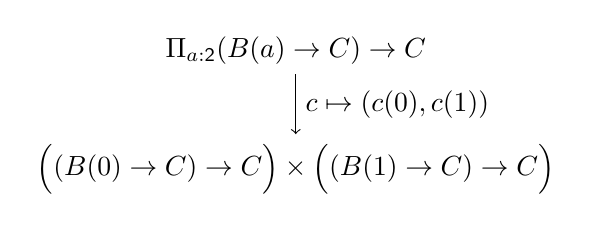
\begin{tikzpicture}
\node (N0) at (0,12) {$\prd{a:\Bool} (B(a) \to C) \to C$};
\node (N1) at (0,10.5) {$\Big((B(0) \to C) \to C\Big) \times \Big((B(1) \to C) \to C\Big)$};
\draw[->] (N0) -- node[right]{$c \mapsto (c(0), c(1))$} (N1);
\end{tikzpicture}
\end{center}
Since $B(0) = 0$, the type $B(0) \to C$ is contractible, with center $\lam{b:B(0)} \abort(C,F \; b)$. We thus have an equivalence
\begin{center}
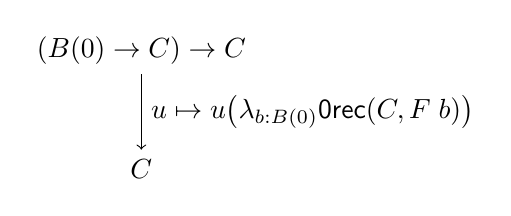
\begin{tikzpicture}
\node (N0) at (0,12) {$(B(0) \to C) \to C$};
\node (N1) at (0,10.5) {$C$};
\draw[->] (N0) -- node[right]{$u \mapsto u\big(\lam{b:B(0)} \abort(C,F \; b)\big)$} (N1);
\end{tikzpicture}
\end{center}
Since $B(1) = 1$, the map $x \mapsto \lam{\_}\; x$ is an equivalence from $C$ to $B(1) \to C$. Thus, we have an equivalence
\begin{center}
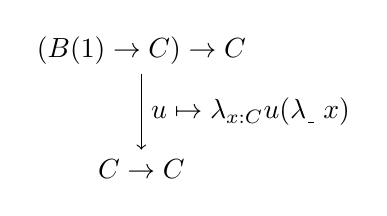
\begin{tikzpicture}
\node (N0) at (0,12) {$(B(1) \to C) \to C$};
\node (N1) at (0,10.5) {$C \to C$};
\draw[->] (N0) -- node[right]{$u \mapsto \lam{x:C} u(\lam{\_} \; x)$} (N1);
\end{tikzpicture}
\end{center}
Putting this all together, we see that the map 
\[ (C,c) \mapsto \Big(C,c\big(0,\lam{b} \abort(C,F \; b)\big),\lam{x:C} c(1, \lam{\_} \; x)\Big)\] 
is an equivalence from $\WAlg_{\UU_i}(A,B)$ to $\NatAlg_{\UU_i}$.
\end{proof}

\begin{lemma}
For any $\X : \WAlg_{\UU_i}(A,B)$ there is an equivalence
\[ \WFibAlgToNatFibAlg_{\UU_j} : \WFibAlg_{\UU_j}(A,B) \; \X \to \NatFibAlg_{\UU_j}(\WAlgToNatAlg_{\UU_i}(\X)) \]
\end{lemma}
\begin{proof}
Let an algebra $(C,c) : \WAlg_{\UU_i}(A,B)$ be given and fix $E : C \to \UU_j$. We have an equivalence
\begin{center}
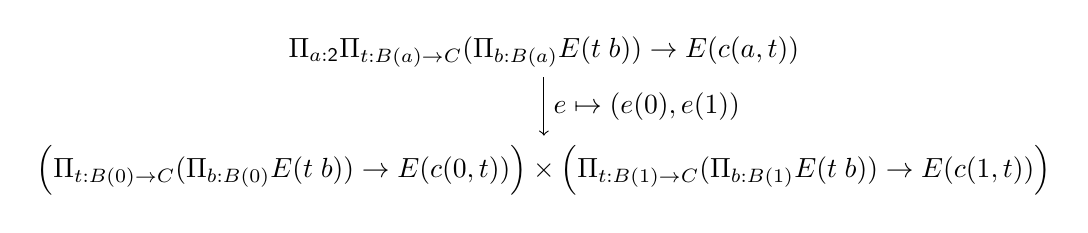
\begin{tikzpicture}
\node (N0) at (0,12) {$\prd{a:\Bool}\prd{t:B(a)\to C} (\prd{b:B(a)} E(t\;b)) \to E(c(a,t))$};
\node (N1) at (0,10.5) {$\Big(\prd{t:B(0)\to C} (\prd{b:B(0)} E(t\;b)) \to E(c(0,t))\Big) \times \Big(\prd{t:B(1)\to C} (\prd{b:B(1)} E(t\;b)) \to E(c(1,t))\Big)$};
\draw[->] (N0) -- node[right]{$e \mapsto (e(0), e(1))$} (N1);
\end{tikzpicture}
\end{center}
Since $B(0) = 0$, the type $B(0) \to C$ is contractible, with center $\lam{b:B(0)} \abort(C,F \; b)$. Likewise, $\prd{b:B(0)} E(\abort(C,F \; b))$ is contractible, with center 
$\lam{b:B(0)} \abort\big(E(\abort(C,F \; b)), F \;b\big)$. We thus have equivalences
\begin{center}
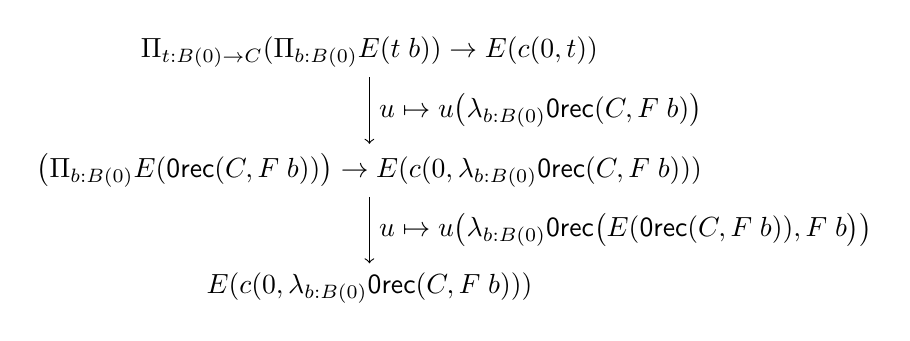
\begin{tikzpicture}
\node (N0) at (0,12) {$\prd{t:B(0)\to C} (\prd{b:B(0)} E(t\;b)) \to E(c(0,t))$};
\node (N1) at (0,10.5) {$\big(\prd{b:B(0)} E(\abort(C,F \; b))\big) \to E(c(0,\lam{b:B(0)} \abort(C,F \; b)))$};
\node (N2) at (0,9) {$E(c(0,\lam{b:B(0)} \abort(C,F \; b)))$};
\draw[->] (N0) -- node[right]{$u \mapsto u\big(\lam{b:B(0)} \abort(C,F \; b)\big)$} (N1);
\draw[->] (N1) -- node[right]{$u \mapsto u\big(\lam{b:B(0)} \abort\big(E(\abort(C,F \; b)), F \;b\big)\big)$} (N2);
\end{tikzpicture}
\end{center}
Since $B(1) = 1$, the map $x \mapsto \lam{\_}\; x$ is an equivalence from $C$ to $B(1) \to C$. Likewise, for any $x:C$ the map $y \mapsto \lam{\_}\; y$  is an equivalence from $E(x)$ to $B(1) \to E(x)$. Thus, we have equivalences
\begin{center}
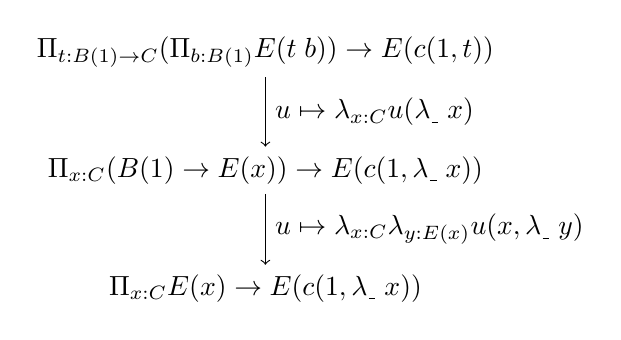
\begin{tikzpicture}
\node (N0) at (0,12) {$\prd{t:B(1)\to C} (\prd{b:B(1)} E(t\;b)) \to E(c(1,t))$};
\node (N1) at (0,10.5) {$\prd{x:C} (B(1) \to E(x)) \to E(c(1,\lam{\_} \; x))$};
\node (N2) at (0,9) {$\prd{x:C} E(x) \to E(c(1,\lam{\_} \; x))$};
\draw[->] (N0) -- node[right]{$u \mapsto \lam{x:C} u(\lam{\_} \; x)$} (N1);
\draw[->] (N1) -- node[right]{$u \mapsto \lam{x:C} \lam{y:E(x)} u(x,\lam{\_} \; y)$} (N2);
\end{tikzpicture}
\end{center}
Putting this all together, we see that the map 
\[ (E,e) \mapsto \Big(E,e\big(0,\lam{b} \abort(C,F \; b), \lam{b} \abort(E(\abort(C,F \; b)), F \;b)\big),\lam{x:C} \lam{y:E(x)} e(1, \lam{\_} \; x, \lam{\_} \; y)\Big)\] 
is an equivalence from $\WFibAlg_{\UU_j}(A,B) \; (C,c)$ to $\NatFibAlg_{\UU_j}(\WAlgToNatAlg_{\UU_i} \; (C,c))$.
\end{proof}

\begin{lemma}
For any $\X : \WAlg_{\UU_i}(A,B)$ and $\Y : \WFibAlg_{\UU_j}(A,B) \; \X$ we have
\[ \WFibHom \; \X \; \Y \;\; \simeq \;\; \NatFibHom \; \big(\WAlgToNatAlg_{\UU_i}(\X)\big) \; \big(\WFibAlgToNatFibAlg_{\UU_j}(\Y)\big) \]
\end{lemma}
\begin{proof}
Let algebras $(C,c) : \WAlg_{\UU_i}(A,B)$ and $(E,e) : \WFibAlg_{\UU_j}(A,B) \; (C,c)$ be given and fix $f : \prd{x:C} E(x)$. We have an equivalence
\begin{center}
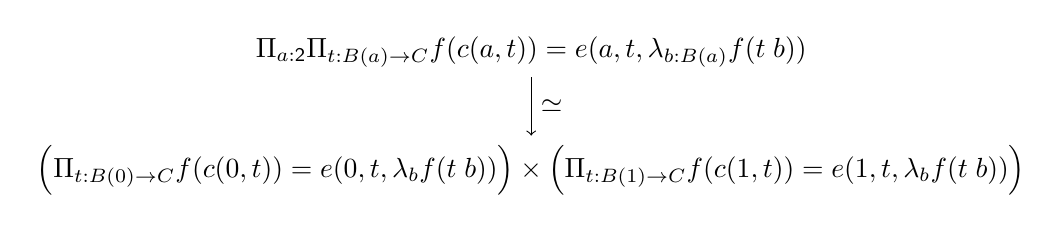
\begin{tikzpicture}
\node (N0) at (0,12) {$\prd{a:\Bool}\prd{t:B(a)\to C} f(c(a,t)) = e(a,t,\lam{b:B(a)} f(t\;b))$};
\node (N1) at (0,10.5) {$\Big(\prd{t:B(0)\to C} f(c(0,t)) = e(0,t,\lam{b} f(t\;b))\Big) \times \Big(\prd{t:B(1)\to C} f(c(1,t)) = e(1,t,\lam{b} f(t\;b))\Big)$};
\draw[->] (N0) -- node[right]{$\simeq$} (N1);
\end{tikzpicture}
\end{center}
Since $B(0) = 0$, the type $B(0) \to C$ is contractible, with center $\lam{b:B(0)} \abort(C,F \; b)$. Furthermore, since all functions out of $\zero$ are equal, we have
\[\lam{b} f(\abort(C,F \; b)) = \lam{b} \abort(E(\abort(C,F \; b)), F \;b)\] This implies the following equivalences:
\begin{center}
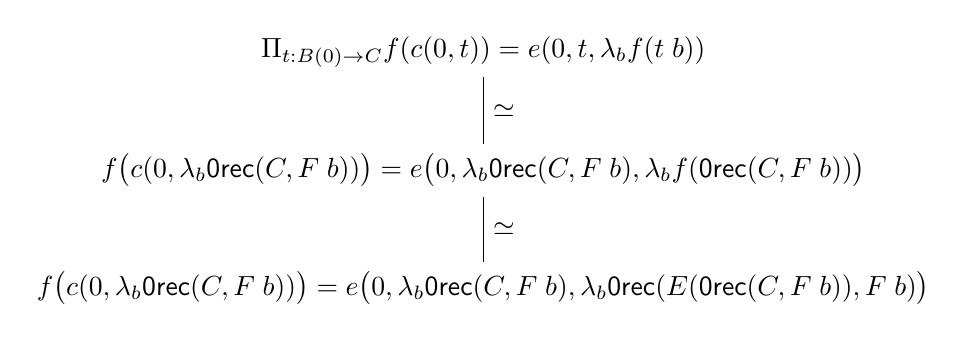
\begin{tikzpicture}
\node (N0) at (0,12) {$\prd{t:B(0)\to C} f(c(0,t)) = e(0,t,\lam{b} f(t\;b))$};
\node (N1) at (0,10.5) {$f\big(c(0,\lam{b} \abort(C,F \; b))\big) = e\big(0,\lam{b} \abort(C,F \; b),\lam{b} f(\abort(C,F \; b))\big)$};
\node (N2) at (0,9) {$f\big(c(0,\lam{b} \abort(C,F \; b))\big) = e\big(0,\lam{b} \abort(C,F \; b),\lam{b} \abort(E(\abort(C,F \; b)), F \;b)\big)$};
\draw[-] (N0) -- node[right]{$\simeq$} (N1);
\draw[-] (N1) -- node[right]{$\simeq$} (N2);
\end{tikzpicture}
\end{center}
Since $B(1) = 1$, the map $x \mapsto \lam{\_}\; x$ is an equivalence from $C$ to $B(1) \to C$. Thus, we have an equivalence
\begin{center}
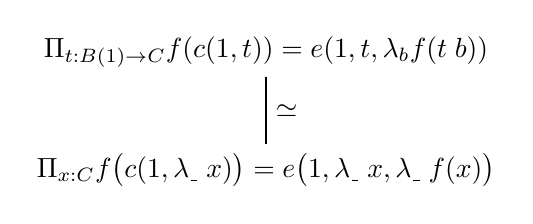
\begin{tikzpicture}
\node (N0) at (0,12) {$\prd{t:B(1)\to C} f(c(1,t)) = e(1,t,\lam{b} f(t\;b))$};
\node (N1) at (0,10.5) {$\prd{x:C} f\big(c(1,\lam{\_} \; x)\big) = e\big(1,\lam{\_} \; x,\lam{\_} \; f(x)\big)$};
\draw[-] (N0) -- node[right]{$\simeq$} (N1);
\end{tikzpicture}
\end{center}
This finishes the proof.
\end{proof}

\begin{corollary}
For any $\X : \WAlg_{\UU_i}(A,B)$ and $\Y : \WAlg_{\UU_j}(A,B)$ we have
\[ \WHom \; \X \; \Y \;\; \simeq \;\; \NatHom \; \big(\WAlgToNatAlg_{\UU_i}(\X)\big) \; \big(\WAlgToNatAlg_{\UU_j}(\Y)\big) \]
\end{corollary}

\begin{corollary}
For any $\X : \NatAlg_{\UU_i}$ we have
\begin{alignat*}{4}
& \HasNatRec_{\UU_j}(\X) & \;\; \simeq \;\; & \HasWRec_{\UU_j}(\WAlgToNatAlg_{\UU_i}^{-1}(\X)) \\
& \HasNatInd_{\UU_j}(\X) & \;\; \simeq \;\; & \HasWInd_{\UU_j}(\WAlgToNatAlg_{\UU_i}^{-1}(\X)) \\
& \HasNatRecUniq_{\UU_j}(\X) &  \simeq \;\; & \HasWRecUniq_{\UU_j}(\WAlgToNatAlg_{\UU_i}^{-1}(\X)) \\
& \HasNatIndUniq_{\UU_j}(\X) & \simeq \;\; &  \HasWIndUniq_{\UU_j}(\WAlgToNatAlg_{\UU_i}^{-1}(\X)) \\
& \IsNatHInit_{\UU_j}(\X) & \simeq \;\; & \IsWHInit_{\UU_j}(\WAlgToNatAlg_{\UU_i}^{-1}(\X))
\end{alignat*}
\end{corollary}

\begin{corollary}\label{lem:NatMainInt}
In $\Hint$, the following conditions on an algebra $\X : \NatAlg_{\UU_i}$ are equivalent:
\begin{enumerate}
\item $\X$ satisfies the induction principle on the universe $\UU_j$
\item $\X$ satisfies the recursion and recursion uniqueness principles on the universe $\UU_j$
\item $\X$ is homotopy-initial on the universe $\UU_j$  
\end{enumerate}
for $j \geq i$. In other words, we have \[ \HasNatInd_{\UU_j}(\X)  \;\; \simeq \;\; \HasNatRec_{\UU_j}(\X) \times \HasNatRecUniq_{\UU_j}(\X) \;\; \simeq \;\; \IsNatHInit_{\UU_j}(\X) \]
provided $j \geq i$. Furthermore, all 3 conditions are mere propositions.
\end{corollary}

We can thus characterize the type $\nat$ using the universal property of initiality as follows.
\begin{corollary}\label{lem:NatInitInt}
In $\Hint$ with natural numbers, the algebra $(\nat,\z,\suc(-)) : \NatAlg_{\UU_0}$ is homotopy-initial on any universe $\UU_j$.
\end{corollary}

\begin{corollary}\label{lem:NatCharInt}
In $\Hint$ extended with an algebra $\X : \NatAlg_{\UU_0}$ which is homotopy-initial on any universe $\UU_j$, the type $\nat$ with propositional computation rules is definable. 
\end{corollary}
\begin{proof}
We have an algebra $\cdot \vdash \X : \NatAlg_{\UU_0}$ such that for any $j$, there exists a term $\cdot \vdash h_j  : \IsNatHInit_{\UU_j}(\X)$. Since the requirement $j \geq 0$ always holds, Cor.~\ref{lem:NatMainInt} implies that for any $j$, we have a term $\cdot \vdash r_j : \HasNatInd_{\UU_j}(\X)$. This implies that the type $\nat$ with propositional computation rules is definable.
\end{proof}

%Finally, let us observe that the definition of a type representing the second number class as a W-type,
%as discussed in~\cite{MartinLofP:inttt}, carries over equally well. Indeed, one
%now must represent type-theoretically a signature with three operations: the first of arity zero, 
%the second of arity one, and the third of arity $\nat$. For the first two we can proceed exactly as
%before, while for the third there is no need to prove auxiliary results on adjoint homotopy 
%equivalences. As before, the second number class supports an h-initial algebra structure for the corresponding polynomial functor $P(X) = \mathsf{1} + X + (\nat \rightarrow X)$.
%Again, the formal development of this result in Coq can be found in~\cite{AwodeyS:indtht}.

%Finally, the case $\List(A)$ of finite lists of elements of type $A$ can be treated analogously, in terms of the polynomial functor 
%\[
%P(X) = \mathsf{1} + A\!\times\! X\, .
%\]
%%
%We again refer to~\cite{AwodeyS:indtht} for details.


\section{Old Part}
\subsection{Extensional W-types}\label{section:extW}
%%%%%%%%%%%%%%%%%%%%%%%


\noindent 
We briefly recall the theory of W-types in fully extensional type theories. Let us begin by recalling
the rules for W-types from~\cite{MartinLofP:inttt}. To state them more conveniently, we sometimes
write~$W$ instead of $(\W x : A) B(x)$. 

\smallskip

\begin{itemize}
\item $\W$-formation rule.
\[
\begin{prooftree}
 A : \type \qquad
 x : A \vdash B(x) : \type
 \justifies
 (\W x : A) B(x) : \type
\end{prooftree}
\]
\item $\W$-introduction rule.
\[
\begin{prooftree}
a:A \qquad
t : B(a) \rightarrow W
\justifies
\wsup(a, t): W
\end{prooftree}
\]
\item $\W$-elimination rule.
\[
 \begin{prooftree}
 \hspace{-1ex} \begin{array}{l}
 w : W \vdash C(w) : \type \\ 
 x:A \, , u:  B(x) \rightarrow W \, ,  v : (\Pi y : B(x)) C(u(y))  \vdash \\ 
   \qquad c(x,u,v) : C(\wsup(x,u))
   \end{array}
 \justifies
w : W \vdash    \wrec(w,c) : C(w) 
\end{prooftree}
\]
\item $\W$-computation rule.
\[
 \begin{prooftree}
 \hspace{-1ex} \begin{array}{l}
 w : W \vdash C(w) : \type \\ 
 x:A \, , u:  B(x) \rightarrow W \, ,  v : (\Pi y : B(x)) C(u(y))  \vdash \\ 
   \qquad c(x,u,v) : C(\wsup(x,u))
   \end{array}
 \justifies
 \begin{array}{l} 
x : A, u : B(x) \rightarrow W \vdash 
\wrec(\wsup(x,u), c) = \\ 
  \qquad c(x,u, \lambda y. \wrec(u(y), c)) : C(\wsup(x,u)) \, .
\end{array}
\end{prooftree}
\]
\end{itemize}

\noindent


\medskip

W-types can be seen informally as the free algebras for signatures
with operations of possibly infinite arity, but no equations. Indeed, the premisses 
of the formation rule above can be thought of as specifying a signature that has the elements of~$A$ 
as operations and in which the arity of~ $a : A$ is the cardinality of the type~$B(a)$. Then, the introduction rule specifies the canonical way of forming an element of the free algebra, and the elimination rule can be seen as the propositions-as-types translation of the appropriate induction principle.

In extensional type theories, this informal description can easily be turned into a precise
mathematical characterization. To do so, let us use the theory $\Hext$ obtained
by extending $\Hint$ with the reflection rule in~\eqref{equ:collapse}. Let $\mathcal{C}(\Hext)$ be the category with
types as objects and elements $f : A \rightarrow B$ as maps, in which two maps are
considered equal if and only if they are definitionally equal. The premisses of the introduction
rule determines the \emph{polynomial endofunctor} $P : \mathcal{C}(\Hext) \rightarrow \mathcal{C}(\Hext)$
defined by 
\[
    P(X) \defeq (\Sigma x : A ) (B(x) \rightarrow X) \, .
\]
A $P$-algebra is a pair consisting of a type $C$ and a function $s_C : PC \rightarrow C$, called 
the structure map of the algebra. The formation rule gives us an object $W \defeq (\W x : A)
B(x)$ and the introduction rule (in combination with the rules for $\Pi$-types
and $\Sigma$-types) provides a structure map
\[
s_W : PW \rightarrow W \, .
\]
The elimination rule, on the other hand, states that in order for the projection $\pi_1 \colon C \rightarrow W$, where
$C \defeq (\Sigma w {\, : \, } W) C(w)$, to have a section $s$, as in the diagram
\[
\xymatrix{
& C  \ar[d]^{\pi_1} \\
W \ar[ru]^{s} \ar[r]_{1_W} & W, 
}
\]
it is sufficient for the type $C$ to have a $P$-algebra structure over $W$. Finally, the computation rule states that the section $s$ given by the elimination rule is also a $P$-algebra homomorphism. 

The foregoing elimination rule implies what we call the \emph{simple} $\W$-elimination rule:
\[
\begin{prooftree}
C : \type  \qquad
 x : A, v : B(x) \rightarrow C \vdash c(x,v) : C
 \justifies
w : W \vdash \wrecs(w,c) :  C
\end{prooftree}
\]
This can be recognized as a recursion principle for maps from $W$ into $P$-algebras, since
the premisses of the rule describe exactly a type $C$ equipped with a structure map $s_C 
: PC  \rightarrow C$. For this special case of the elimination rule, the corresponding computation rule again states that the function
\[
\lambda w. \wrecs(w,c) : W \rightarrow C \, ,
\] 
where $c(x,v) = s_C(\pair(x,v))$ for $x : A$ and $v : B(x) \rightarrow C$, is a $P$-algebra homomorphism.
Moreover, this homomorphism can then be shown to be definitionally unique using the elimination
rule, the principle of function extensionality and the reflection rule.  The converse implication also holds: one can derive the general $\W$-elimination rule from the simple elimination rule and the following $\eta$-rule
%
\begin{equation*}
\begin{prooftree}
\begin{array}{l}
C : \type  \qquad w : W \vdash h(w) : C \\ 
x : A, v : B(x) \rightarrow C \vdash c(x,v) : C\\
x:A \, , u:  B(x) \rightarrow W  \vdash h\left(\wsup(x,u)) = c(x,\lambda y. hu(y)\right) : C
  \end{array}
 \justifies
w : W \vdash  h(w) =  \wrecs(w,c) :  C
\end{prooftree}
\end{equation*}
%
stating the uniqueness of the $\wrecs$ term among algebra maps. 
Overall, we therefore have that  in 
$\Hext$ induction and recursion are interderivable: 
\[
\begin{array}{ccc}
\text{\underline{\myemph{Induction}}} & \Leftrightarrow & \text{\underline{\myemph{Recursion}}}\\[1ex]
\text{$\W$-elimination} & & \text{Simple $\W$-elimination}\\
\text{$\W$-computation} &&  \text{Simple $\W$-computation + $\eta$-rule} 
\end{array}
\]

Finally, observe that what we are calling recursion is equivalent to the statement that the
type $W$, equipped with the structure map $s_W : PW \rightarrow W$ 
is the initial $P$-algebra. Indeed, assume the simple elimination rule, the simple computation
rule and the $\eta$-rule; then for any $P$-algebra $s_C : PC\rightarrow C$, there is a 
function $f : W \rightarrow C$ by the simple elimination rule, which is a homomorphism by the computational 
rule, and is the unique such homomorphism by the $\eta$-rule.  The converse implication from initiality to recursion is just as direct. Thus, in the extensional theory, to have an initial algebra for the endofunctor $P$ is the same thing
as having a type~$W$ satisfying the introduction, elimination and computation rules above.  Section~\ref{section:intW} will be devoted to generalizing this equivalence to the setting of Homotopy Type Theory.

%%%%%%%%%%%%%%%%%%%%%%%%%%%%%%%%%%%%%
\subsection{Inductive types as W-types}

\noindent To conclude our review, recall that in extensional type theory, many inductive types can be reduced to W-types.  We mention the following  examples, among many others (see \cite{MartinLofP:inttt}, \cite{DybjerP:repids}, \cite{GoguenH:inddtw}, \cite{MoerdijkI:weltc}, \cite{GambinoN:weltdp}, \cite{AbbottM:concsp}):
\begin{enumerate}
\item \emph{Natural numbers}. \label{extnatW}
The usual rules for $\nat$ as an inductive type can be derived from its formalization as the following W-type. Consider the signature with two operations, one of which has arity $0$ and one of which has arity $1$; it is presented type-theoretically by a dependent type with corresponding polynomial functor (naturally isomorphic to)
\[
P(X) = \mathsf{1} + X \, ,
\]
%
and the natural numbers $\nat$ together with the canonical element $0:\nat$ and the successor function $s : \nat\rightarrow\nat$ form an initial $P$-algebra
\[
(0, s) : \mathsf{1} + \nat \rightarrow \nat\, .
\]
%
\item \emph{Second number class.}
As shown in~\cite{MartinLofP:inttt}, the second number class can be obtained as a W-type determined by the polynomial functor 
\[
P(X) = \mathsf{1} + X + (\nat \rightarrow X) \, .
\]
This has algebras with three operations, one of arity $0$, one of arity $1$, and one of arity (the cardinality of) $\nat$.
%
%\item \emph{Lists.}  The type $\List(A)$ of finite lists of elements of type $A$ can be built as a W-type determined by the polynomial functor 
%\[
%P(X) = \mathsf{1} + A\!\times\! X \, .
%\]
%We refer to \cite{xxx} % need a reference here !
% for details.
\end{enumerate}

\smallskip

%%%%%%%%%%%%%%%%%%%%%%%%%
\subsection{Intensional W-types}\label{section:intW}
%%%%%%%%%%%%%%%%%%%%%%%%%

\noindent We begin with an example which serves to illustrate, in an especially simple case, some aspects of our theory.  The type of Boolean truth values is not a W-type, but it can be formulated as an inductive type in the familiar way by means of  formation, introduction, elimination, and computation rules.  It then has an ``up to homotopy" universal property of the same general kind as the one that we shall formulate in section \ref{subsection:main} below for W-types, albeit in a simpler form.

%%%%%%%%%%%%%%%%%%%%%%%%%%
\subsection{Preliminary example}\label{subsection:prelimex}

\noindent The standard rules for the type $\Bool$ given in~\cite[Section~5.1]{NordstromB:marltt}
can be stated equivalently as follows.

\begin{itemize}
\item $\Bool$-formation rule.
\[
 \Bool : \type \, .
 \]
\item $\Bool$-introduction rules.
\[
0 : \Bool \, ,  \qquad  1 : \Bool \, .
\]
\item $\Bool$-elimination rule.\smallskip
\[
\begin{prooftree}
x : \Bool \vdash C(x) : \type \qquad
c_0 : C(0) \qquad
c_1 : C(1) 
\justifies
x: \Bool \vdash \boolrec(x, c_0, c_1) : C(x) 
\end{prooftree}
\]
\item $\Bool$-computation rules. 
\begin{equation*}
\begin{prooftree}
x : \Bool \vdash C(x) : \type \qquad
c_0 : C(0) \qquad
c_1 : C(1) 
\justifies
\left\{
\begin{array}{c} 
 \boolrec(0, c_0, c_1)  =  c_0 : C(0)  \, , \\
 \boolrec(1, c_0, c_1)  =  c_1 : C(1) \, .
 \end{array}
\right.
\end{prooftree}
 \end{equation*} 
\end{itemize}

Although these rules are natural ones to consider in the intensional setting, they do not imply a strict universal property. For example, given a type $C$ and elements $c_0, c_1 : 
C$, the function $\lambda x . \boolrec(x, c_0,c_1) : \Bool \rightarrow C$ cannot  be shown to be definitionally unique among the functions $f :  
\Bool \rightarrow C$ with the property that $f(0)=c_0 : C$ and $f(1)=c_1 : C$.  
The best that one can do by using $\Bool$-elimination over a suitable identity type, and function extensionality, is to show that it is unique among all such maps up to an identity term, which itself is unique up to a higher identity, which in turn is unique up to \ldots. This sort of weak $\omega$-universality, which apparently involves infinitely much data, can nonetheless be captured directly within the system of type theory (without resorting to coinduction) using ideas from higher category theory. To do so, let us define a \emph{$\Bool$-algebra} to be a type $C$ equipped with two elements
$c_0 \, , c_1 : C$. Then, a \emph{weak homomorphism} of $\Bool$-algebras
$(f, p_0, p_1) : (C, c_0,c_1)\rightarrow (D,d_0,d_1)$  
consists of a  function $f : C\rightarrow D$ together with identity terms 
\[
p_0 :  \id{D}(f (c_0) ,d_0) \, , \qquad p_1 :   \id{D}(f (c_1), d_1) \, .
\]
This is a \emph{strict homomorphism} when $f (c_0) = d_0 : D$, $f (c_1) = d_1 : D $ and the identity terms $p_0$ and $p_1$ are the corresponding reflexivity terms.  We can then define the type of weak homomorphisms from $(C, c_0,c_1)$ to $(D,d_0,d_1)$ by letting
\begin{multline*}
\BoolAlg [ (C, c_0,c_1), (D,d_0,d_1) \big] \defeq \\
 (\Sigma f: C \rightarrow D) \Id(f (c_0), d_0) \times\id{D}(f (c_1), d_1) \, .
\end{multline*}
The weak universality condition on the $\Bool$-algebra $(\Bool, 0, 1)$ that we seek can now be determined as follows. 

\begin{definition} \label{thm:boolhinitial}
A $\Bool$-algebra $(C, c_0,c_1)$ is \emph{homotopy-initial} if for any $\Bool$-algebra $(D,d_0,d_1)$, the type 
\[
\BoolAlg \big[ (C, c_0,c_1), (D,d_0,d_1)\big]
\] 
is contractible.
\end{definition}

\noindent The notion of homotopy initiality, or h-initiality for short, captures in a precise way the informal idea that there is essentially one weak algebra homomorphism $(\Bool, 0, 1) \rightarrow (C,c_0,c_1)$.  Moreover, h-initiality can be shown to follow from the rules of inference for $\Bool$ stated above.  Indeed, the  computation rules for $\Bool$ stated above
 evidently make the function
\[
\lambda x . \boolrec(x, c_0,c_1) : \Bool \rightarrow C
\]
into a \emph{strict} algebra map, a stronger condition than is required for h-initiality.  Relaxing these 
definitional equalities to propositional ones, we arrive at the following rules.

\smallskip

\noindent
\begin{itemize}
\item Propositional $\Bool$-computation rules.
\[
\begin{prooftree}
x : \Bool \vdash C(x) : \type \qquad
c_0 : C(0) \qquad
c_1 : C(1) 
\justifies
\left\{
\begin{array}{c} 
\boolcomp_0(c_0, c_1) :  \id{C(0)} \big(\boolrec(0, c_0, c_1), c_0)  \, , \\ 
\boolcomp_1(c_0, c_1)  : \id{C(1)} \big(\boolrec(1, c_0, c_1), c_1)  \, .
\end{array}
\right.
\end{prooftree}
\]
\end{itemize}

\smallskip

This variant is not only still sufficient for h-initiality, but also necessary, as we state precisely in the following.

\begin{proposition} \label{prop:2hinitial}
Over the type theory $\Hint$, the formation, introduction, elimination, and propositional computation rules
for $\Bool$ are equivalent to the existence of a homotopy-initial $\Bool$-algebra.
\end{proposition}
%%
\begin{proof}[Proof sketch] 
Suppose we have a type $\Bool$ satisfying the stated rules.  Then clearly $(\Bool, 0, 1)$ is a $\Bool$-algebra; to show that it is h-initial, take any $\Bool$-algebra $(C,c_0,c_1)$.  By elimination with respect to the constant family $C$ and the elements $c_0$ and $c_1$, we have the map $\lambda x . \boolrec(x, c_0,c_1) : \Bool \rightarrow C$, which is a weak algebra homomorphism by the propositional computation rules.  Thus we obtain a term $h:\BoolAlg\big[ (\Bool, 0, 1), (C, c_0,c_1)\big]$.  Now given any $k:\BoolAlg\big[ (\Bool, 0, 1), (C, c_0,c_1)\big]$, we need a term of type $\id{}(h,k)$.  This term follows from a propositional $\eta$-rule, which is derivable by $\Bool$-elimination over a suitable identity type.

Conversely, let $(\Bool, 0, 1)$ be an h-initial $\Bool$-algebra.  To prove elimination, let $x:\Bool \vdash C(x):\type$ with $c_0 : C(0)$ and $ c_1 : C(1)$ be given, and consider the $\Bool$-algebra $(C', c'_0, c'_1)$ defined by:
%
\begin{align*}
C' &\defeq (\Sigma x: \Bool)C(x) \, , \\
c'_0 &\defeq \pair(0, c_0) \, , \\
c'_1 &\defeq \pair(1, c_1)\, .
\end{align*}
%
Since $\Bool$ is h-initial, there is a map $r : \Bool\rightarrow C'$ with identities $p_0:\id{}(r  0, c'_0)$ and $p_1:\id{}(r  1, c'_1)$.  Now, we would like to set 
$$\boolrec(x, c_0, c_1) = \pi_2 (r x) : C(x),$$
 where $\pi_2$ is the second projection from $C'=(\Sigma x: \Bool)C(x)$.  But recall that in general 
 $\pi_2(z) : C(\pi_1(z))$, and so (taking the case $x=0$) we have $\pi_2(r   0) : C(\pi_1(r   0))$ rather than the required $\pi_2(r   0) {\, : \, } C(0)$; that is, since it need not be that $\pi_1(r   0) = 0$, the term $\pi_2(r   0)$ has the wrong type to be $\boolrec(0, c_0, c_1)$.  However, we can show that $$\pi_1: (\Sigma x: \Bool)C(x)\rightarrow \Bool$$ is a weak homomorphism, so that the composite $\pi_1\circ r : (\Bool, 0, 1)\rightarrow (\Bool, 0, 1)$ must be propositionally equal to the identity homomorphism $1_\Bool : (\Bool, 0, 1)\rightarrow (\Bool, 0, 1)$, by the contractibility of $\BoolAlg \big[ (\Bool, 0, 1), (\Bool, 0, 1)\big]$.  Thus there is an identity term $p : \id{}(\pi_1\circ r, 1_\Bool)$, along which we can transport using $p_! : C(\pi_1( r   0)) \rightarrow C(0)$, thus taking $\pi_2(r   0 ) : C(\pi_1 (r   0))$ to the term  $p_! ( \pi_2( r   0) ) :C(0)$ of the correct type.  We can then set
\[
\boolrec(x, c_0, c_1) = p_! (\pi_2 (r x)) : C(x)
\]
to get the required elimination term.  The computation rules follow by a rather lengthy calculation.
\end{proof}

%%
Proposition~\ref{prop:2hinitial} is the analogue in Homotopy Type Theory of the characterization of 
$\Bool$ as a strict coproduct $1+1$ in extensional type theory. It makes precise the rough idea that, 
in intensional type theory, $\Bool$ is a kind of homotopy coproduct or weak $\omega$-coproduct 
in the weak $\omega$-category $\mathcal{C}(\Hint)$ of types, terms, identity terms, higher identity terms, \ldots.  
It is worth emphasizing that h-initiality is a purely type-theoretic notion; despite having an obvious semantic interpretation, it is formulated in terms of inhabitation of specific, definable types.  Indeed, Proposition~\ref{prop:2hinitial} and its proof have been completely formalized in the Coq proof assistant~\cite{AwodeyS:indtht}.  

\begin{remark} A development entirely analogous to the foregoing can be given for the type
$\nat$ of natural numbers. In somewhat more detail, one introduces the notions of a $\nat$-algebra and 
of a weak homomorphism of $\nat$-algebras. Using these, it is possible to define the notion of
a homotopy-initial $\nat$-algebra, analogue to that of a homotopy-initial
$\Bool$-algebra in Definition~\ref{thm:boolhinitial}. With these definitions in place, one can prove an equivalence between the formation, introduction, elimination and propositional computation rules for $\nat$ and the existence of a homotopy-initial $\nat$-algebra. 
Here, the propositional computation rules are formulated like those above, \emph{i.e.} by replacing the definitional equalities in the conclusion of the usual computation rules~\cite[Section~5.3]{NordstromB:marltt} with propositional equalities. 
 We do not pursue this further here, however, since $\nat$ can also be presented as a W-type, as we discuss in section \ref{subsec:define} below.
\end{remark}

%%%%%%%%%%%%%%%%%%%%%%%%%%
\subsection{The main theorem}\label{subsection:main}

\noindent Although it is more elaborate to state (and difficult to prove) owing to the presence of 
recursively generated data, our main result on  W-types is analogous to 
the foregoing example in the following respect: rather than being strict initial algebras, as in the 
extensional case, weak W-types are instead homotopy-initial algebras.  This fact can again be stated 
entirely syntactically, as an equivalence between two sets of rules:  the 
formation, introduction, elimination, and propositional computation rules (which we spell
out below) for W-types, and the existence of an h-initial algebra, in the appropriate sense.  Moreover, as in the simple case of the type $\Bool$, the proof of the equivalence is again entirely constructive. 

The required definitions in the current setting are as follows. Let us assume that
\[
x:A \vdash B(x) : \type \, ,
\]
and define the associated polynomial functor as before: 
\begin{equation}
\label{eq:polyfunc}
PX = (\Sigma x : A) (B(x) \rightarrow X) \, .
\end{equation}
(Actually, this is now functorial only up to propositional equality, but this change makes no difference in what follows.)
By definition, a $P$-algebra is a type $C$ equipped a function
$s_C :  PC \rightarrow C$. For $P$-algebras $(C,s_C)$ and $(D,s_D)$, a \emph{weak 
homomorphism} between them $(f, s_f) : (C, s_C) \rightarrow (D, s_D)$
consists of a function $f : C \rightarrow D$ and an identity proof
\[
s_f : \id{PC \rightarrow D}\big( f \circ s_C \, ,  s_{D} \circ Pf \big) \, ,
\]
where $Pf : PC\rightarrow PD$ is the result of the easily-definable action of $P$ on $f: C \rightarrow D$. Such an algebra homomorphism can be represented suggestively in the form:
\[
\xymatrix{
 PC \ar[d]_{s_C} \ar[r]^{Pf}  \ar@{}[dr]|{s_f} &  PD \ar[d]^{s_D}\\
C \ar[r]_{f}   & D }
\] 
Accordingly, the type of weak algebra maps is defined by
\begin{multline*}
\Palg
\big[ (C,s_C), (D, s_D)  \big]
 \defeq   \\
(\Sigma f:  C \rightarrow D) \, \Id(f\circ s_C, s_D\circ Pf) \, .
\end{multline*}


\begin{definition} 
A $P$-algebra $(C, s_C)$ is \emph{homotopy-initial} if for every $P$-algebra $(D, s_D)$, the type 
$$\Palg \big[ (C, s_C), (D, s_D) \big]$$ of weak algebra maps is contractible.
\end{definition} 


\begin{remark} 
The notion of h-initiality captures a universal property in which the usual conditions of existence and uniqueness  are replaced by conditions of existence and uniqueness up to a system of higher and higher identity proofs. To explain this, let us fix a $P$-algebra  $(C,s_C)$ and assume that it is homotopy-initial. Then, given any 
$P$-algebra~$(D,s_D)$, there is a weak homomorphism $(f,s_f) : (C,s_C) \rightarrow (D,s_D)$, since
the type of weak maps from $(C,s_C)$ to $(D,s_D)$, being contractible, is inhabited. Furthermore, for any weak map $(g,s_g) : (C,s_C) \rightarrow (D,s_D)$, the
contractibility of the type of weak maps  implies that there is an identity proof 
\[
 p  : \Id\big( (f,s_f), (g, s_g) \big) \, , 
\]
witnessing the uniqueness up to propositional equality of the homomorphism $(f,s_f)$. But it
is also possible to prove that the identity proof $p$ is unique up to propositional equality. Indeed, since 
$(f,s_f)$ and $(g,s_g)$ are elements of a contractible type, the identity type $\Id( (f,s_f), (g, s_g) )$ 
is also contractible, as observed in Remark~\ref{thm:idcontrcontr}. Thus, if we have another 
identity proof $q : \Id( (f,s_f), (g, s_g) )$, there will be an identity term $\alpha : \Id(p,q)$, which is again
essentially unique, and so on.  It should also be pointed out that, just as strictly initial algebras are unique
up to isomorphism, h-initial algebras are unique up to weak equivalence. It then follows from
the Univalence axiom that two h-initial algebras are propositionally equal, a fact that we mention only by the way. Finally, we note that there is also a homotopical version of Lambek's Lemma, asserting that the structure map of an h-initial algebra is itself a weak equivalence, making the algebra a \emph{homotopy fixed point} of the associated polynomial functor. The reader can work out the details from the usual proof and the definition of  h-initiality, or consult~\cite{AwodeyS:indtht}.
\end{remark}

\medskip

The deduction rules that characterize homotopy-initial algebras are
obtained from the formation, introduction, elimination and computation rules for W-types 
stated in Section~\ref{section:extW} by simply replacing the $\W$-computation rule with the
following rule, that we call the propositional $\W$-computation rule.

\smallskip

\begin{itemize} 
\item Propositional $\W$-computation rule.
\[
\begin{prooftree}
\begin{array}{l} 
w : W \vdash C(w) : \type \\ 
\hspace{-1ex}
\begin{array}{c} 
x : A, u : B(x) \rightarrow W, v : (\Pi y : B(x)) C(u(y)) \vdash \\ 
c(x,u,v) : C(\wsup(x,u))  
\end{array}
\end{array}
\justifies
\begin{array}{l} 
x : A, u : B(x) \rightarrow W \vdash 
\wcomp(x,u,c) :  \\
\qquad \Id
\big(
\wrec(\wsup(x,u), c), c(x,u,\lambda y.\wrec( u(y), c )
\big)
\end{array}
\end{prooftree}
\]
\end{itemize}



 \begin{remark}\label{thm:wtypesinvariance}
One interesting aspect of this group of rules, to which we shall refer as the \emph{rules for homotopical
W-types}, is that, unlike the standard rules for W-types, they are invariant under propositional
equality. To explain this  more precisely, let us work in a type theory with a type universe $\UU$ closed
under all the forms of types of $\Hint$ and W-types. Let $A : \UU$, $B : A
\rightarrow \UU$ and define $W \defeq (\W x : A) B(x)$. The invariance of
the rules for homotopy W-types under propositional equality can now be expressed by saying that if we have a type $W' : \UU$  and an identity proof $p : \id{U}(W, W')$, then the $\Id$-elimination rule 
implies that  $W'$ satisfies the same rules as $W$, in the sense that there are definable terms playing the role of the primitive  constants that
appear in the rules for $W$.
\end{remark}

We can now state our main result. Its proof has been formalized in the Coq system,
and the proof scripts are available at~\cite{AwodeyS:indtht}; thus we provide only an outline of the proof. 

\begin{theorem}\label{theorem:main}
Over the type theory $\Hint$, 
the rules for homotopical W-types
are equivalent to the existence of homotopy-initial algebras for polynomial functors.
\end{theorem}

%%%%%
\begin{proof}[Proof sketch] 
The two implications are proved separately.
First, we show that the rules for homotopical W-types imply the existence
of homotopy-initial algebras for polynomial functors. Let us assume that
$x : A \vdash B(x) : \type$ 
and consider the associated polynomial functor $P$, defined as in~\eqref{eq:polyfunc}.
Using the $\W$-formation rule, we define $W \defeq (\W x : A) B(x)$ and using
the $\W$-introduction rule we define a structure map $s_W : PW \rightarrow W$,
exactly as in the extensional theory. We claim that the algebra $(W, s_W)$ is
h-initial. So, let us consider another algebra $(C,s_C)$ and prove that the type $T$ 
of weak homomorphisms from $(W, s_W)$ to $(C,s_C)$ is contractible. To do
so, observe that the $\W$-elimination rule and the propositional $\W$-computation
rule allow us to define a weak homomorphism $(f, s_f) : (W, s_W) \rightarrow (C, s_C)$, 
thus showing that $T$ is inhabited. Finally, it is necessary to show that for every weak homomorphism $(g, s_g) : (W, s_W) \rightarrow (C, s_C)$, there
is an identity proof 
\begin{equation}
\label{equ:prequired}
p : \Id( (f,s_f), (g,s_g) ) \, .
\end{equation}
This uses the fact that, in general, a type of the form $\Id( (f,s_f), (g,s_g) )$,
is weakly equivalent to the type of what we call \emph{algebra $2$-cells}, whose canonical
elements are pairs of the form $(e, s_e)$, where $e : \Id(f,g)$ and $s_e$ is a higher identity proof witnessing the propositional equality between the identity proofs represented by the following pasting diagrams:
\[
\xymatrix{
PW \ar@/^1pc/[r]^{Pg}   \ar[d]_{s_W} \ar@{}[r]_(.52){s_g}  & PD \ar[d]^{s_D}  \\
W \ar@/^1pc/[r]^g  \ar@/_1pc/[r]_f  \ar@{}[r]|{e} & D } \qquad
\xymatrix{
PW \ar@/^1pc/[r]^{Pg}   \ar[d]_{s_W}   \ar@/_1pc/[r]_{Pf} \ar@{}[r]|{Pe}
& PD \ar[d]^{s_D}  \\
W  \ar@/_1pc/[r]_f  \ar@{}[r]^{s_f} & D }
\]
In light of this fact, to prove that there exists a term as in~\eqref{equ:prequired}, it is 
sufficient to show that there is an algebra 2-cell 
\[
(e,s_e) : (f,s_f) \Rightarrow (g,s_g) \, .
\]
The identity proof $e : \Id(f,g)$ is now constructed by function extensionality and
$\W$-elimination so as to guarantee the existence of the required identity
proof $s_e$. 

\smallskip

For the converse implication, let us assume that the polynomial functor associated
to the judgement $x : A \vdash B(x) : \type$ 
%\[
%x : A \vdash B(x) : \type
%\] 
has an h-initial algebra $(W,s_W)$. To derive the $\W$-formation rule, we 
let  $(\W x {\, : \, } A) B(x) \defeq W$. The $\W$-introduction rule is equally simple to
derive; namely, for $a : A$ and $t \colon B(a) \rightarrow W$,  we define $\wsup(a,t) : W$ as the 
result of applying the structure map $s_W \colon PW \rightarrow W$ to $\pair(a,t) : PW$.
For the $\W$-elimination rule, let us assume its premisses and in particular that $w : W \vdash C(w) : \type$.
%\[
%w : W \vdash C(w) : \type \, .
%\]
Using the other premisses, one shows that the type $C \defeq (\Sigma w : W) C(w)$
can be equipped with a structure map $s_C : PC \rightarrow C$. By the h-initiality of $W$,
we obtain a weak homomorphism $(f, s_f) : (W, s_W) \rightarrow (C, s_C)$. Furthermore,
the first projection $\pi_1 : C \rightarrow W$ can be equipped with the structure of a weak 
homomorphism, so that we obtain a diagram of the form
\[
\xymatrix{
PW \ar[r]^{Pf} \ar[d]_{s_W}  & PC \ar[d]^{s_C}  \ar[r]^{P \pi_1}  & PW  \ar[d]^{s_W}  \\
W \ar[r]_f  & C \ar[r]_{\pi_1}  & W \, .}
\]
But the identity function $1_W : W \rightarrow W$ has a canonical structure of a weak
algebra homomorphism and so, by the contractibility of the type of weak homorphisms
from $(W,s_W)$ to itself, there must be an identity proof between the composite
of $(f,s_f)$ with $(\pi_1, s_{\pi_1})$ and $(1_W, s_{1_W})$. This implies, in particular,
that there is an identity proof $p : \Id( \pi_1 \circ f, 1_W)$. 
%\[
%p : \Id( \pi_1 \circ f, 1_W) \, .
%\]
Since $(\pi_2 \circ f) w : C( (\pi_1 \circ f) w)$, we can define
\[
\wrec(w,c) \defeq
p_{\, ! \,}( ( \pi_2 \circ  f)   w )   : C(w) 
\]
where the transport $p_{\, ! \,}$ is defined via $\Id$-elimination over the dependent type
\[
u : W \rightarrow W \vdash C ( u (w)) : \type \, .
\]
The verification of the propositional $\W$-computation rule is a rather long calculation,
involving several lemmas concerning the naturality properties of operations of the form $p_{\, ! \,}$.
\end{proof}
%%%%%

%%%%%%%%%%%%%%%%%%%%%%%%%%
\subsection{Definability of inductive types}\label{subsec:define}

\noindent We conclude this section by indicating how the limited form of extensionality that is assumed in the type theory~$\Hint$, namely the principle of function extensionality, allows us to overcome the obstacles in defining various inductive types as W-types mentioned at the end of Section~\ref{section:extW}, provided that both are understood in the appropriate homotopical way, \emph{i.e.} with all types being formulated with propositional computation rules. 

Consider first the paradigmatic case of the type of natural numbers. To define it as a W-type, we work in an extension of the type theory $\Hint$ with
\begin{itemize}
\item formation, introduction, elimination and propositional computation rules 
for types $\mathsf{0}$, $\mathsf{1}$ and $\mathsf{2}$ that have zero, one and two canonical elements,
respectively; 
\item the rules for homotopy W-types, as stated above;
\item rules for a type universe $\UU$ reflecting all the forms of types of $\Hint$, W-types, and
$\mathsf{0}$, $\mathsf{1}$ and $\mathsf{2}$.
\end{itemize}
In particular, the rules for $\mathsf{2}$ are those given in Section~\ref{subsection:prelimex}.
We then proceed as follows. We begin by setting $A =\mathsf{2}$, as in the extensional case.  
We then define a dependent type
\[
x : A \vdash B(x) : \UU
\]
by $\mathsf{2}$-elimination, so that the propositional $\mathsf{2}$-computation rules give us 
propositional equalities
\[
 p_0 : \id{U}( \mathsf{0}, B(0)) \, , \qquad
 p_1 : \id{U}( \mathsf{1}, B(1)) \, .
\]
Because of the invariance of the rules for $\mathsf{0}$ and $\mathsf{1}$ under propositional
equalities (as observed in Remark~\ref{thm:wtypesinvariance}), we can then derive that the types~$B(0)$ and~$B(1)$ satisfy rules analogous to those for $\mathsf{0}$ and $\mathsf{1}$, respectively. This allows us to show that the type 
\[
\nat \defeq (\W x : A) B(x)
\]
satisfies the introduction, elimination and propositional computation rules for the type of natural numbers. 
The proof of this fact proceeds essentially as one would expect, but to derive the propositional computation rules it
is useful to observe that for every type $X : \UU$, there are adjoint homotopy equivalences,
in the sense of Definition \ref{thm:weq}, between the types $\mathsf{0}  \rightarrow X$ and $\mathsf{1}$, 
and between $\mathsf{1} \rightarrow X$ and $X$. Indeed, the propositional identities witnessing 
the triangular laws are useful in the verification of the propositional computation rules for $\nat$. For 
details, see the formal development in Coq provided in~\cite{AwodeyS:indtht}.  Observe that as a W-type, $\nat$ is therefore also an h-initial algebra for the equivalent polynomial functor $P(X) = \mathsf{1}+ X$, as expected.

Finally, let us observe that the definition of a type representing the second number class as a W-type,
as discussed in~\cite{MartinLofP:inttt}, carries over equally well. Indeed, one
now must represent type-theoretically a signature with three operations: the first of arity zero, 
the second of arity one, and the third of arity $\nat$. For the first two we can proceed exactly as
before, while for the third there is no need to prove auxiliary results on adjoint homotopy 
equivalences. As before, the second number class supports an h-initial algebra structure for the corresponding polynomial functor $P(X) = \mathsf{1} + X + (\nat \rightarrow X)$.
Again, the formal development of this result in Coq can be found in~\cite{AwodeyS:indtht}.

%Finally, the case $\List(A)$ of finite lists of elements of type $A$ can be treated analogously, in terms of the polynomial functor 
%\[
%P(X) = \mathsf{1} + A\!\times\! X\, .
%\]
%%
%We again refer to~\cite{AwodeyS:indtht} for details.




\section{Future work}\label{section:future}
The treatment of W-types presented here is part of a larger investigation of general inductive types in Homotopy Type Theory.  We sketch the projected course of our further research.

\begin{enumerate}
\item  In the setting of  extensional type theory, Dybjer \cite{DybjerP:repids} showed that every strictly positive definable functor can be represented as a polynomial functor, so that all such inductive types are in fact W-types.  This result should generalize to the present setting in a straightforward way.

\item Also in the extensional setting, Gambino and Hyland~\cite{GambinoN:weltdp} showed that 
general tree types~\cite{PeterssonK:setcis}~\cite[Chapter~16]{NordstromB:promlt}, viewed as 
initial algebras for general polynomial functors, can be constructed from W-types in
locally cartesian closed categories, using equalizers. We expect this result to carry over to the present setting as well, using $\id{}$-types in place of equalizers.

\item In \cite{VoevodskyV:notts} Voevodsky has shown that all inductive types of the Predicative Calculus of Inductive Constructions can be reduced to the following special cases:
\begin{itemize}
\item $\mathsf{0}$,\ $\mathsf{1}$,\ $A+B$,\  $(\Sigma x : A)B(x)$,
\item $\id{A}(a,b)$,
\item general tree types.
\end{itemize}
Combining this with the foregoing, we expect to be able to extend our Theorem \ref{theorem:main} to the full system of predicative inductive types underlying Coq.
\end{enumerate}

\noindent Finally, one of the most exciting recent developments in Univalent Foundations is the 
idea of Higher Inductive Types (HITs), which can also involve identity terms in their signature~\cite{LumsdaineP:higit,ShulmanM:higit}.   This allows for algebras with equations between terms, like associative laws, coherence laws, etc.; but the really exciting aspect of HITs comes from the homotopical interpretation of identity terms as paths.  Viewed thus, HITs should permit direct formalization of many basic geometric spaces and constructions, such as the unit interval $I$; the spheres $S^n$, tori, and cell complexes; truncations, such as the [bracket] types \cite{AwodeyS:prot}; various kinds of quotient types; homotopy (co)limits; and many more fundamental and fascinating objects of geometry not previously captured by type-theoretic formalizations.  Our investigation of conventional inductive types in the homotopical setting should lead to a deeper understanding of these new and important geometric analogues. 

\begin{acks}
We would like to thank Vladimir Voevodsky and Michael Warren for helpful discussions
on the subject of this paper. In particular, Vladimir Voevodsky suggested a simplification of the 
proof that the rules for homotopical W-types imply h-initiality.

Steve Awodey gratefully acknowledges the support of the National Science Foundation, Grant DMS-1001191
 and the Air Force OSR, Grant 11NL035.
Nicola Gambino is grateful for the support of the Institute for Advanced Study, where
he worked on this project. This work was supported by the National Science Foundation 
under agreement No.\ DMS-0635607. Any opinions, findings and conclusions or recommendations
expressed in this material are those of the authors and do not necessarily reflect the views of
the National Science Foundation.
Kristina Sojakova is grateful for the support of CyLab at Carnegie
Mellon under grants DAAD19-02-1-0389 and W911NF-09-1-0273 from the Army
Research Office.
\end{acks}

\bibliographystyle{ACM-Reference-Format-Journals}
\bibliography{references}
                        
\received{}{}{}

\end{document}